% File project.tex
%% Style files for ACL 2021
\documentclass[11pt,a4paper]{article}
\usepackage[hyperref]{acl2021}
\usepackage{times}
\usepackage{booktabs}
\usepackage{todonotes}
\usepackage{latexsym}
\usepackage{float}
\usepackage{caption}
\usepackage{subcaption}
\usepackage{enumitem}
\usepackage[normalem]{ulem}
\renewcommand{\UrlFont}{\ttfamily\small}
% This is not strictly necessary, and may be commented out,
% but it will improve the layout of the manuscript,
% and will typically save some space.
\usepackage{etoolbox} 
\AtBeginEnvironment{itemize}{\setlength\parskip{0pt}}
\AfterEndEnvironment{itemize}{\vspace*{-\dimexpr\parskip\relax}}
\usepackage{microtype}
\usepackage{bbm}

% \titlespacing*{\section}
% {0pt}{0pt}{0pt}
% \titlespacing*{\subsection}
% {0pt}{0pt}{0pt}
% \titlespacing*{\subsubsection}
% {0pt}{0pt}{0pt}

\aclfinalcopy 

\newcommand\BibTeX{B\textsc{ib}\TeX}

\newcommand{\vp}[1]{\textcolor{blue}{\bf\small [#1 --AS]}}
\newcommand{\ar}[1]{\textcolor{green}{\bf\small [#1 --AS]}}
\newcommand{\as}[1]{\textcolor{red}{\bf\small [#1 --AS]}}

\title{Toward Stronger Priors and Better Grounding: An Instruction Following and Navigation Approach}

% \title{Toward Stronger Priors and Better Grounding for Instruction Following and Navigation}

\author{
  Andrew Singh\thanks{\hspace{4pt}Everyone Contributed Equally -- Alphabetical order} \hspace{2em} Ankit Ramchandani$^*$ \hspace{2em} Vashisth Parekh$^*$ \\
  \texttt{\{andrewsi, aramchan, vparekh\}@andrew.cmu.edu}
  }

\date{}

\begin{document}
\maketitle
\begin{abstract}
\end{abstract}

For an artificially intelligent agent, performing everyday tasks given natural language instructions and egocentric visual input is very difficult. Recently, ALFRED, an instruction following and navigation dataset for household tasks, was proposed to advance the state of the art in embodied intelligence. Agents in ALFRED have to complete long horizon tasks with non-reversible actions, understand complex interactions between vision, language, and their own actions, and generalize to unseen objects and environments. While several models have been proposed to solve this challenging benchmark, all of them perform very poorly on both seen and unseen validation/test splits compared to humans. Through both quantitative and qualitative assessment, we argue that even the best models are still highly primitive. We note that an important shortcoming of all previous models is that they hope that incredibly rich and sophisticated representations will automatically emerge in their models without designing/enforcing them. To this end, we propose a novel model that can disentangle between explicit and implicit forms of representations and context, thereby significantly reducing the learning load of each component. While we do not have all final results yet, we show that our model is capable of fitting the training dataset significantly faster while using much fewer parameters than all previous models. Given more time, we are hopeful that we would be able to achieve strong results with our model.
\section{Introduction}
A holy grail of the machine learning community is to create an intelligent agent that can understand and execute natural language instructions from a human. Clearly, this is very difficult to achieve with current methods because it requires complex interaction and grounding between the natural language instructions the agent receives, and the visual observations it makes at any time step. Recently, an instruction following and navigation dataset, ALFRED \cite{shridhar2020alfred}, was released with the aim to push the state of the art in embodied artificial intelligence, and multimodal machine learning. Specifically, the agent in the ALFRED environment is given a high level goal statement, and a sequence of low level step by step instructions to complete a task. At each time step, the agent has access to these natural language instructions, and the current egocentric visual input, and is expected to produce a action, and an interaction mask of the object of interest. This benchmark is uniquely challenging because it contains non-reversible actions and state changes, long sequences, and complex interactions between language instructions and visual input. The dataset also places strong emphasis on generalization: the agent's performance is tested on an ``unseen'' split using novel instances of objects, novel layouts, and novel scenes.

Several models have been proposed \cite{shridhar2020alfred, corona2020modularity, singh2020moca, Storks2021AreWT} to solve the ALFRED task. However, their performance has been surprisingly low: the best ALFRED model published so far, MOCA \cite{singh2020moca}, can successfully solve only 22\% of tasks in the seen split, and a mere 5.3\% of tasks in the unseen test split. As we discuss later, simple qualitative analysis of the proposed models reveals that they are significantly primitive and do not have the same understanding a human would when completing the same task. For example, we note (with video links) that many agents just keep going in circles, and cannot recover from simple mistakes made early in the trajectory, which reflects that current agents cannot even remember their past actions, let alone performing well on the entire instruction following task.

\begin{figure}[H]
\centering
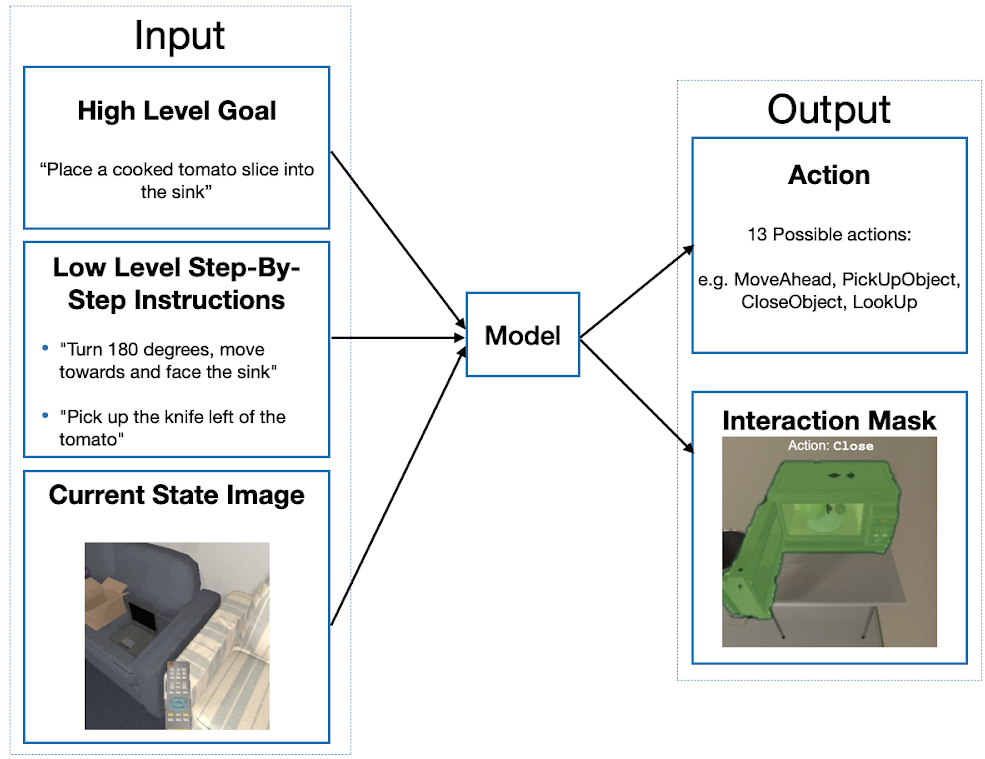
\includegraphics[width=\linewidth]{figures/intro_figure.png}
\caption{A visualization of the ALFRED task. At each timestep, the agent receives a high-level goal, a series of low-level instructions, and an ego-centric image as input, and it must predict the next action and, if necessary, corresponding interaction mask as output.}
\label{fig:intro-figure}
\end{figure}

Motivated by these observations (which are backed more strongly in subsequent sections), our main hypotheses is that current models rely on emergent properties just too much without providing any direct enforcement to make those properties emerge in the first place. For example, most methods just rely on the hidden state of some multimodal LSTM to keep track of the agent's state. However, as we argue in detail later, ``keeping track'' involves a lot of things: understanding high level goal, instructions, visual input, grounding different modalities in each other, recalling action and interaction histories, etc. We believe it is unlikely that such a rich representation will emerge automatically in the hidden state without any enforcement. In fact, we know it does not often because, as said earlier, the agent sometimes just keeps going in circles.

To this end, we propose a novel model which more clearly grounds language in vision, and encodes stronger priors by disentangling between explicit and implicit forms of context. We present initial experiments on our model which show that it has significant potential to achieve strong performance using about half the parameters that MOCA \cite{singh2020moca} uses, and significantly less training time (i.e. gradient steps) compared to any prior models.

\section{Related Work and Background}
\label{sec:rel-work}
\subsection{Models for ALFRED}
\label{ssec:alf}
Several approaches have been recently proposed that demonstrate improved performance on the ALFRED benchmark over the baseline introduced in \newcite{shridhar2020alfred}. The baseline architecture consists of a CNN to encode  visual input at each timestep, a bi-LSTM to encode language directives, and a decoder LSTM to infer the action at each timestep while attending over the language encoding. \newcite{corona2020modularity} add separate modules for each \emph{subgoal type} (e.g., GOTO, PICKUP) to the baseline architecture and then use a high-level controller to choose which module to execute at each step. \newcite{singh2020moca} propose a vision module for generating interaction masks and an action module for predicting actions, with the vision module first predicting the class of the object of interest and then generating the pixel-wise interaction mask given the predicted object class. \newcite{Storks2021AreWT} address ALFRED's long action sequences by training the model to execute one subgoal at a time rather than all subgoals at once, and they address the agent's poor navigation performance by augmenting the agent's perception with additional viewing angles.

Unlike methods that learn a direct mapping from observations to actions end-to-end, \newcite{Saha2021AMV} propose a modular framework that learns from unaligned or weakly aligned data as opposed to requiring expert demonstrations. Their mapping module includes a novel mapping scheme based on graph convolutional networks \cite{kipf2016semi} for improved navigation, and their language module leverages a pre-trained model to perform joint intent detection and slot filling on the language directives. \newcite{Shridhar2020ALFWorldAT} propose a new environment to address the challenge of generalizing to unseen tasks. They align tasks in ALFRED with a purely textual environment, TextWorld \cite{Ct2018TextWorldAL}, allowing agents to first learn in an abstract setting in order to generalize better in the embodied setting. 


\subsection{Related Tasks}
\paragraph{Vision and Language Navigation}
\label{ssec:vln}
While ALFRED requires navigation and interaction with objects based on visual and language input, a related task is vision and language based navigation (VLN). \newcite{fried2018speaker} propose a policy where a follower model, which produces a step-by-step action sequence from visual and textual input, generates multiple trajectories, and the one most likely to match with the natural language description was chosen by a speaker model.

\newcite{wani2020multion} perform several experiments on a long-horizon navigation task in a realistic 3D setting to empirically show that using a semantic map-like memory can significantly boost navigation performance. \newcite{hao2020learning} pre-train their model on image-text-action triplets in a self-supervised manner. Their model is able to generalize better in unseen environments, improving the SOTA in the Room-to-Room task. \newcite{majumdar2020improving} improve VLN performance by using a visiolinguistic transformer based model that scores the compatibility between an instruction and a particular visual scene. 

\paragraph{Embodied Question Answering}
\label{ssec:eqa}
Embodied Question Answering \cite{Das2018EmbodiedQA} (EmbodiedQA) is a related task in which an agent spawns at a random location in a 3D environment and is asked a question about an object. To correctly answer, the agent must navigate the environment and gather information through egocentric vision about the object and its surroundings. 

\newcite{Das2018EmbodiedQA} propose an approach with a two-step navigation module: a planner that selects actions and a controller that executes those actions a variable number of times. Their agent is initialized via imitation learning and then fine-tuned via reinforcement learning. \newcite{Das2018NeuralMC} improve upon this approach by introducing a high-level policy that proposes compositional sub-goals to be executed by sub-policies and trained in a similar fashion. \newcite{Yu2019MultiTargetEQ} generalize the EmbodiedQA task to answering questions about \textit{multiple} objects, and propose a modular approach that converts the question to executable sub-programs, executes these sub-programs to guide the agent, selects relevant observations along the agent's path, and uses these observations to predict the final answer.

\subsection{Relevant ML Methods}
\paragraph{Multimodal Alignment}
\label{ssec:mmml}
In the ALFRED task, the agent receives all natural language instructions at the beginning of the episode but receives visual observations at each time-step. It is imperative for the agent to align the natural language directives with its current visual observation so that it can spot objects of interest \cite{baltruvsaitis2018multimodal}.

\newcite{Chen2004Grounding} use a graphical model to align objects in egocentric images with spoken words. \newcite{mei2015listen} use a bi-LSTM with a multi-level aligner to map instructions with navigational actions. \newcite{ma2019selfmonitoring} propose a visual textual co-grounding alignment mechanism and a corresponding progress monitor. They used the hidden state from the previous timestep of their LSTM to generate textual and visual grounding, which helps their agent decide which action to take next. Similarly, \newcite{wang2019reinforced} use an LSTM to predict actions and include an attention mechanism on visual and textual input based on the current hidden state of the LSTM. \newcite{ke2019tactical} use attention mechanism over language to compute how the previous action aligned with the description.

% \paragraph{Generalization in Multimodal Settings}
% \as{Do we need this section?}
% The ALFRED dataset includes \textit{unseen} splits of validation and test data that aim to measure generalization of the learned policy, but multimodal models are more prone to overfitting due to their increased capacity \cite{wang2020makes}. To this end, \newcite{wang2020makes} propose a gradient blending approach that computes optimal blends of modalities based on overfitting behavior, achieving SOTA results on egocentric action tasks similar to ALFRED. \newcite{alet2019modular} present a meta-learning strategy where they separately trained each modular component on related tasks and then combined them to create a more general model that scales across tasks. \newcite{nguyen2018multitask} present an algorithm that uses representation encoders to learn general hierarchical features by fusing visual and semantic representations, and then employs a task-specific decoder for the downstream task.

\paragraph{Imitation Learning}
\label{ssec:rlil}
All known SOTA approaches \cite{singh2020moca, corona2020modularity, Storks2021AreWT} for ALFRED use imitation learning (IL) \cite{hussein2017imitation}, despite IL having several known limitations because the standard i.i.d assumptions are not met \cite{ross2010efficient}. Methods like DAgger \cite{ross2011reduction} that attempt to mitigate the limitations of IL cannot be applied directly because new data cannot be generated on the fly in ALFRED \cite{shridhar2020alfred}. An important technique to improve training with IL was proposed by \cite{salimans2018learning}. They are able to solve Montezuma's Revenge using a single demonstration by training the RL agent to reach the goal by starting from states in the demonstration in reverse order. Since the agent only needs to learn a much shorter sub-task at each step, this approach overcomes the challenge of exploration over long horizons. 


\section{Task Setup and Data}
\subsection{Task Definition}
%Task Definition}
The goal of the ALFRED benchmark is to learn a set of actions in an indoor household setting to perform a task described by natural language. The agent receives high-level and low-level natural language instructions at the beginning of the episode, and can use egocentric visual observation (i.e. access to current RGB image, depth map, and instance segmentation map) at each time step as input. The agent predicts the next action to take, and, if the action involves interaction, a pixel-wise interaction mask of the object of interest. 

% Since current methods \cite{corona2020modularity, singh2020moca, shridhar2020alfred} struggle with generalization to novel objects and environments, we will attempt to primarily focus on improving generalization performance, which is measured by an ``unseen'' split of the test set which contains new environments and objects.

\subsection{Metrics}
The official ALFRED task measures the following metrics for evaluation.
\begin{enumerate}
    \item \textbf{Task Success}: Task success is simply a binary value indicating whether the final states and positions of objects of interest in the trajectory align with expected states (i.e. if task is completed).
    \item \textbf{Goal-Condition Success}: This is the ratio of goal-conditions completed at the end of the episode to the total number of goal-conditions required for task success.
    \item \textbf{Path Weighted Metrics}: We can also compute the path weighted versions of the above metrics. So, if the model takes twice as many actions has the expert, the original task success and goal-conditioned success scores would decrease by half.
\end{enumerate}

% In addition to computing the above metrics on the entire ALFRED task, we will also compute them at the sub-goal level by moving the agent through the expert trajectory before the sub-goal, and then letting it complete the sub-goal. This was also performed by \newcite{shridhar2020alfred}.

Moreover, to better identify performance bottlenecks in ours and other approaches, we propose the following other metrics:

\begin{enumerate}
    \item \textbf{Navigation Object Success (Nav-Obj)} and \textbf{First Navigation Object Success (First-Nav-Obj)}: Navigation Object Success measures the proportion of objects that the agent approached at some point in the episode, out of all the objects the expert interacted with. Here we define ``approached'' as coming within a certain distance and facing the correct orientation. We also record whether the agent could approach just the first object that the expert interacted with, denoted by First Object Navigation Success, due to the fact that poor interaction performance at the first object could adversely affect future navigation performance.
    
    %This metric is important because it more clearly shows whether the agent has at least learned to navigate correctly, which can be measured in a more disentangled manner by only considering navigation to the first object. This is because there will be likely interaction actions before approaching the later objects, making it difficult to reliably attribute credit of future success/failure to navigation alone.

    % Because subsequent actions beyond the first object may involve interaction actions, making it difficult to reliably attribute credit of future success/failure to navigation alone, we also record a True/False of whether the agent approached the first object that the expert interacted with, which we denote First Object Navigation Success. A high value for these metrics indicates that the agent is at least able to successfully navigate to the desired objects, indicating navigation may not necessarily be a performance bottleneck.
    
    \item \textbf{Interaction Success (Int-Succ)}: the proportion of attempted interactions by the agent that were successful (i.e., without an API failure). A high value for this metric indicates that the agent is able to at least successfully predict an appropriate action and interaction mask to interact with objects, even if they may not necessarily be objects that are relevant to the goal.
    
    \item \textbf{Bad Mask Failure Rate (Bad-Mask)}: the proportion of interaction failures that were due to a bad interaction mask. A high value indicates that the primary obstacle to an agent successfully interacting with objects is the interaction mask, while a low value indicates that most of the interaction failures are due to a different reason, such as incorrect action prediction (see item 5: Interaction Action Prediction Success).

    \item \textbf{Unnecessary Interaction Ratio (Unnec-Int)}: Unnecessary Interaction Ratio is defined as the number of  objects the agent interacted with that the expert did not, divided by the number of objects the expert interacted with. A high value will reveal that the agent is interacting with proportionally many objects not relevant to the task, while a low value indicates that the agent is focusing on the objects that are relevant to completing the task.
    
    \item \textbf{Interaction Action Prediction Success (Int-Act-Pred)}: Interaction Action Prediction Success is the fraction of times the model predicts the right interaction action given that it has identified the instance segmentation mask of the correct object. A high value for this metric indicates that once the agent can produce a correct mask, the task of predicting which action to execute is not a bottleneck. A low value suggests that even when the agent is able to produce a correct mask, predicting which action to take is still a significant obstacle to successful interaction.
\end{enumerate}

Note that a recurring theme in most proposed metrics is to measure performance over each aspect needed to solve the task in as much isolation as possible. % For example, we try to measure navigation and interaction performance separately by using NP, IMPP, and IAPP as proposed above.

% In addition to the above base metrics, we also plan to group all metric calculations by task type to understand models at a more fine-grained level.


\section{Previous Models}
\label{sec:prev-models}
\subsection{Baselines and Other Methods}
\label{sssec:baselines}
We plan to use the following methods for comparison purposes, which are cited below and explained in Section \ref{sec:rel-work}.

\begin{itemize}
\item \textbf{Seq-2-Seq PM} \cite{shridhar2020alfred} 
\item \textbf{MOCA} \cite{singh2020moca}
\end{itemize}

% \subsubsection{Current Results}
% See Table \ref{tab:results} for baseline and current results on ALFRED.



\subsection{Automatic evaluation results}
We report our overall results in Table \ref{tab:results}. Additionally, we report results for our proposed intrinsic metrics on the validation set and compare to the baseline model in Table \ref{tab:intrinsic} (left incomplete as results are not yet available). Based on the results of prior models, we make the following observations.

\begin{itemize}
    \item Navigation remains a challenge on unseen data. On the unseen split, even MOCA is unable to navigate to the first relevant object one-third of the times, and only navigates to just over half of the relevant objects throughout the episode. However, the fact that MOCA performs significantly better than the baseline model on the unseen split suggests that the language-guided dynamic filters and obstruction detection that MOCA adds could be beneficial to generalizing navigation to new environments.
    \item Failed interactions are a bottleneck to overall performance on unseen data. We see that even MOCA has just a 24.5\% interacton success rate on the unseen split, while the baseline has a lower 14.8\% success rate. In the case of MOCA, most of these failures (73.7\%) are due to incorrect masks, while just under half are for the baseline. Given that one of MOCA's key contributions is a novel module for object-centric mask prediction, this is somewhat surprising. This could however be explained if the baseline model first encounters other failure modes that MOCA is able to overcome, so the baseline is not able to reach the point where the interaction mask is the bottleneck. Looking further into the data, we find that MOCA attempted nearly $2.5\times$ more interactions than the baseline did, suggesting that perhaps other bottlenecks such as navigation are limiting the baseline's potential for interacting with objects (see item 1).
    \item These models do not focus well on the objects relevant to the goal, interacting with roughly the same number of irrelevant objects as there are relevant objects in the trajectory (shown by the Unnecessary Interaction Ratio of roughly 1 for both models). This suggests that these models are not successfully integrating the language directives with their perceptual inputs to select the objects specified by the directives.
    \item Action prediction remains a significant bottleneck to successful interaction, especially on unseen data. Even after producing a correct interaction mask, MOCA still only predicts the correct interaction action 14\% of the time, and the baseline only 0.8\% of the time, on the unseen split. This suggests that while mask prediction is a significant challenge, an equally (if not more) important task is predicting the correct action to take to interact with the object.
\end{itemize}


\subsection{Qualitative Analysis}
We also ran the baseline and MOCA policy on a few examples to qualitatively analyze the agent's performance. The screen recordings of these examples are uploaded on Google drive, and linked below.

In example 1, titled \href{https://drive.google.com/file/d/1xXIIFGBwzP2QGCXlV4v_YlFTHf9C8228/view?usp=sharing}{Base-Ex1}, the agent has to take a spray bottle from the basin counter and place it on the toilet. Instead, the agent picks up a cloth (placed near the spray bottle) from the basin counter and just moves on the other end of the counter. Note that even though the agent moved correctly to the spray bottle and made only a small mistake (i.e. picked up cloth instead of spray bottle), it could not recover from the mistake, and ended up doing something very different at the end. This highlights a common problem with vanilla imitation learning that the agent cannot recover from small mistakes because that are out of training distribution.

% In the second task, titled \href{https://drive.google.com/file/d/1EBtl4o32FOcBZlhw9CHX83WBGpgXCzCj/view?usp=sharing}{Base-Ex2}, the agent is supposed to pick up two spatulas (one after another) and place them in a drawer. Instead, the agent picks up a loaf (not placed near spatula) of bread and completes a U-turn, which simply highlights how little the agent understands the task.

In the next example, titled \href{https://drive.google.com/file/d/1A790sCe33eKV-MivCO2t5O2DD8Atlh2C/view?usp=sharing}{Base-Ex3}, the agent is supposed to microwave a potato and put it in the fridge. Instead, the agent starts a length trajectory without every picking up the potato: It opens, operates, and closes the microwave repeatedly (sometimes placing nothing inside of it) and then repeatedly opens and closes the fridge (placing nothing inside of it). This example (and many others we have seen) highlight the primitiveness of the agent, and show that the agent is not really learning anything useful, but just operating on statistical co-occurrences: for example, whenever it sees a fridge/microwave, it just repeats a particular action sequence (i.e. open, put object inside, close for fridge or open, put object inside, close, turn on, pick object up, turn off).

The MOCA policy does perform relatively better than the baseline, but the same problems mentioned are noticed. In example \href{https://drive.google.com/file/d/16_FJ3689Mv5dxvu9pU1HZ96QvNm7fCc2/view?usp=sharing}{Moca-Ex4} the agent is asked to slice an apple in the pan with a knife; instead it picks up a fork and travels back and forth in the kitchen. As with baseline, the agent makes a mistake by picking up the fork but is not able to recover from the mistake made early on.

In the next example, \href{https://drive.google.com/file/d/1F400UjTNvMC2pw7HWOOEJ3va-XKUu0nE/view?usp=sharing}{Moca-Ex5} the agent is asked to take a mug, microwave it, and place it on the table across the room again. Unfortunately, the agent simply walks in loops inside the kitchen without even trying to pick up the mug. Similar to the baseline policy, this example reveals that the policy is not really learning anything intuitive, and is not able to attend over the correct objects in long, complex trajectories.

\subsection{Inferences, Interpretations, and Insights}
\label{ssec:insights}
In this section, we analyze the implications of both our quantitative and qualitative results. We noticed that in all proposed ALFRED models, there is a significant reliance on phenomena that the authors expect would automatically emerge without explicit enforcement, and little focus on grounding of different modalities. In the following, we identify concrete instances of such over-reliance on emergent phenomena and little focus on grounding.

\begin{itemize}
    \item \textbf{Too much reliance on LSTM hidden state.} In the original baseline model \cite{shridhar2020alfred} (see Figure \ref{fig:alfred_model}), the LSTM's (shown in green in the figure) hidden state's role is to keep track of current context (as it is used to attend over instructions). However, to perform well in the task, a lot of information needs to be included in the ``context''. For example, ``context'' needs to include some action history, interaction history, instruction understanding, goal understanding, and image understanding with respect to the goal and instruction, among other things. It seems quite unlikely that such a rich representation will automatically emerge in the hidden state, especially without any enforcement. Note that such an argument can be made even for the LSTMs used in the MOCA \cite{singh2020moca} architecture.
    \item \textbf{Little benefit from previous action.} Both MOCA \cite{singh2020moca} and the baseline model \cite{shridhar2020alfred} (see Figures \ref{fig:moca_model} \& \ref{fig:alfred_model}) use the previous action in their model as input to better provide context to the model.  Based on our data analysis, using only the most recent action seems to be ineffective since 60\% of actions are just "MoveAhead"; in other words, 60\% of the time the model cannot extract very meaningful information from the most recent action alone. Furthermore, for interaction actions, keeping track of the action alone does not provide any information about the object that the agent interacted with. Due to these reasons, the burden of the LSTM to maintain an informative context increases even further because all extra information is expected to be stored in its hidden state.
    \item \textbf{Language not grounded in vision.} Both the baseline model and MOCA do not ground language in vision (MOCA grounds vision in language using dynamic filters, but not vice versa). It seems that grounding language in vision (in addition to grounding language in the current context) is essential because visual input directly can tell the model what is visible in the scene, and what to focus on in language accordingly.
\end{itemize}

As we will describe, we attempt to solve all above issues in our model.



\begin{table*}[]
\centering
\resizebox{\textwidth}{!}
{\begin{tabular}{@{}lllllllll@{}}
\toprule
                         & \multicolumn{4}{c}{\textbf{Validation}}                                                                             & \multicolumn{4}{c}{\textbf{Test}}                                                                                   \\
                         & \multicolumn{2}{c}{\textit{Seen}}                        & \multicolumn{2}{c}{\textit{Unseen}}                      & \multicolumn{2}{c}{\textit{Seen}}                        & \multicolumn{2}{c}{\textit{Unseen}}                      \\
Model                    & \multicolumn{1}{c}{Task} & \multicolumn{1}{c}{Goal-Cond} & \multicolumn{1}{c}{Task} & \multicolumn{1}{c}{Goal-Cond} & \multicolumn{1}{c}{Task} & \multicolumn{1}{c}{Goal-Cond} & \multicolumn{1}{c}{Task} & \multicolumn{1}{c}{Goal-Cond} \\ \midrule
Seq2Seq + PM Both \cite{shridhar2020alfred}                & 3.70 (2.10)              & 10.00 (7.00)                  & 0.00 (0.00)              & 6.90 (5.10)                   & 3.98 (2.02)              & 9.42 (6.27)                   & 0.39 (0.80)              & 7.03 (4.26)                   \\
Modular \cite{corona2020modularity}          & \multicolumn{1}{c}{-}    & \multicolumn{1}{c}{-}         & \multicolumn{1}{c}{-}    & \multicolumn{1}{c}{-}         & \multicolumn{1}{c}{-}    & 8.80 (6.30)                   & \multicolumn{1}{c}{-}    & 7.20 (5.70)                   \\
MOCA \cite{singh2020moca}                     & 19.15 (13.60)            & 28.50 (22.30)                 & 3.78 (2.00)              & 13.40 (8.30)                  & 22.05 (15.10)            & 28.29 (22.05)                 & 5.30 (2.72)              & 14.28 (9.99)                  \\
\textbf{Ours}            &                          &                               &                          &                               &                          &                               &                          &                               \\ \midrule
Human                    & \multicolumn{1}{c}{-}    & \multicolumn{1}{c}{-}         & \multicolumn{1}{c}{-}    & \multicolumn{1}{c}{-}         & \multicolumn{1}{c}{-}    & \multicolumn{1}{c}{-}         & 91.00 (85.80)            & 94.50 (87.60)                 \\\bottomrule
\end{tabular}}
\caption{\textbf{Task and Goal-Condition Success Rate.} Corresponding path-weighted metrics are given in parentheses.}
\label{tab:results}
\end{table*}

\begin{table*}[]
\centering
\resizebox{\textwidth}{!}{%
\begin{tabular}{@{}lllllllllllll@{}}
\toprule
                      & \multicolumn{6}{c}{\textit{Seen}}                                                                                                                             & \multicolumn{6}{c}{\textit{Unseen}}                                                                                                      \\ \midrule
Model                 & Nav-Obj                   & First-Nav-Obj               & Int-Succ                  & Bad-Mask             & Unnec-Int & \multicolumn{1}{l|}{Int-Act-Pred} & Nav-Obj                   & First-Nav-Obj               & Int-Succ                & Bad-Mask             & Unnec-Int & Int-Act-Pred \\ \midrule
Seq2Seq + PM Both     & \multicolumn{1}{r}{0.680} & \multicolumn{1}{r}{0.735} & \multicolumn{1}{r}{0.494} & \multicolumn{1}{r}{0.250} & 1.298     & \multicolumn{1}{l|}{0.131}        & \multicolumn{1}{r}{0.283} & \multicolumn{1}{r}{0.322} & \multicolumn{1}{r}{0.148} & \multicolumn{1}{r}{0.437} & 0.809     & 0.008        \\
MOCA                  & \multicolumn{1}{r}{0.778} & \multicolumn{1}{r}{0.838} & \multicolumn{1}{r}{0.470} & \multicolumn{1}{r}{0.617} & 1.103     & \multicolumn{1}{l|}{0.279}        & \multicolumn{1}{r}{0.586} & \multicolumn{1}{r}{0.669} & \multicolumn{1}{r}{0.245} & \multicolumn{1}{r}{0.737} & 1.375     & 0.140        \\
\textbf{Ours}         &                           &                           &                           &                           &           & \multicolumn{1}{l|}{}             &                           &                           &                           &                           &           &              \\\bottomrule
\end{tabular}%
}
\caption{Intrinsic Metrics - Validation.}
\label{tab:intrinsic}
\end{table*}





\section{Approach}
\label{sec:approach}

\begin{figure*}
    \centering
    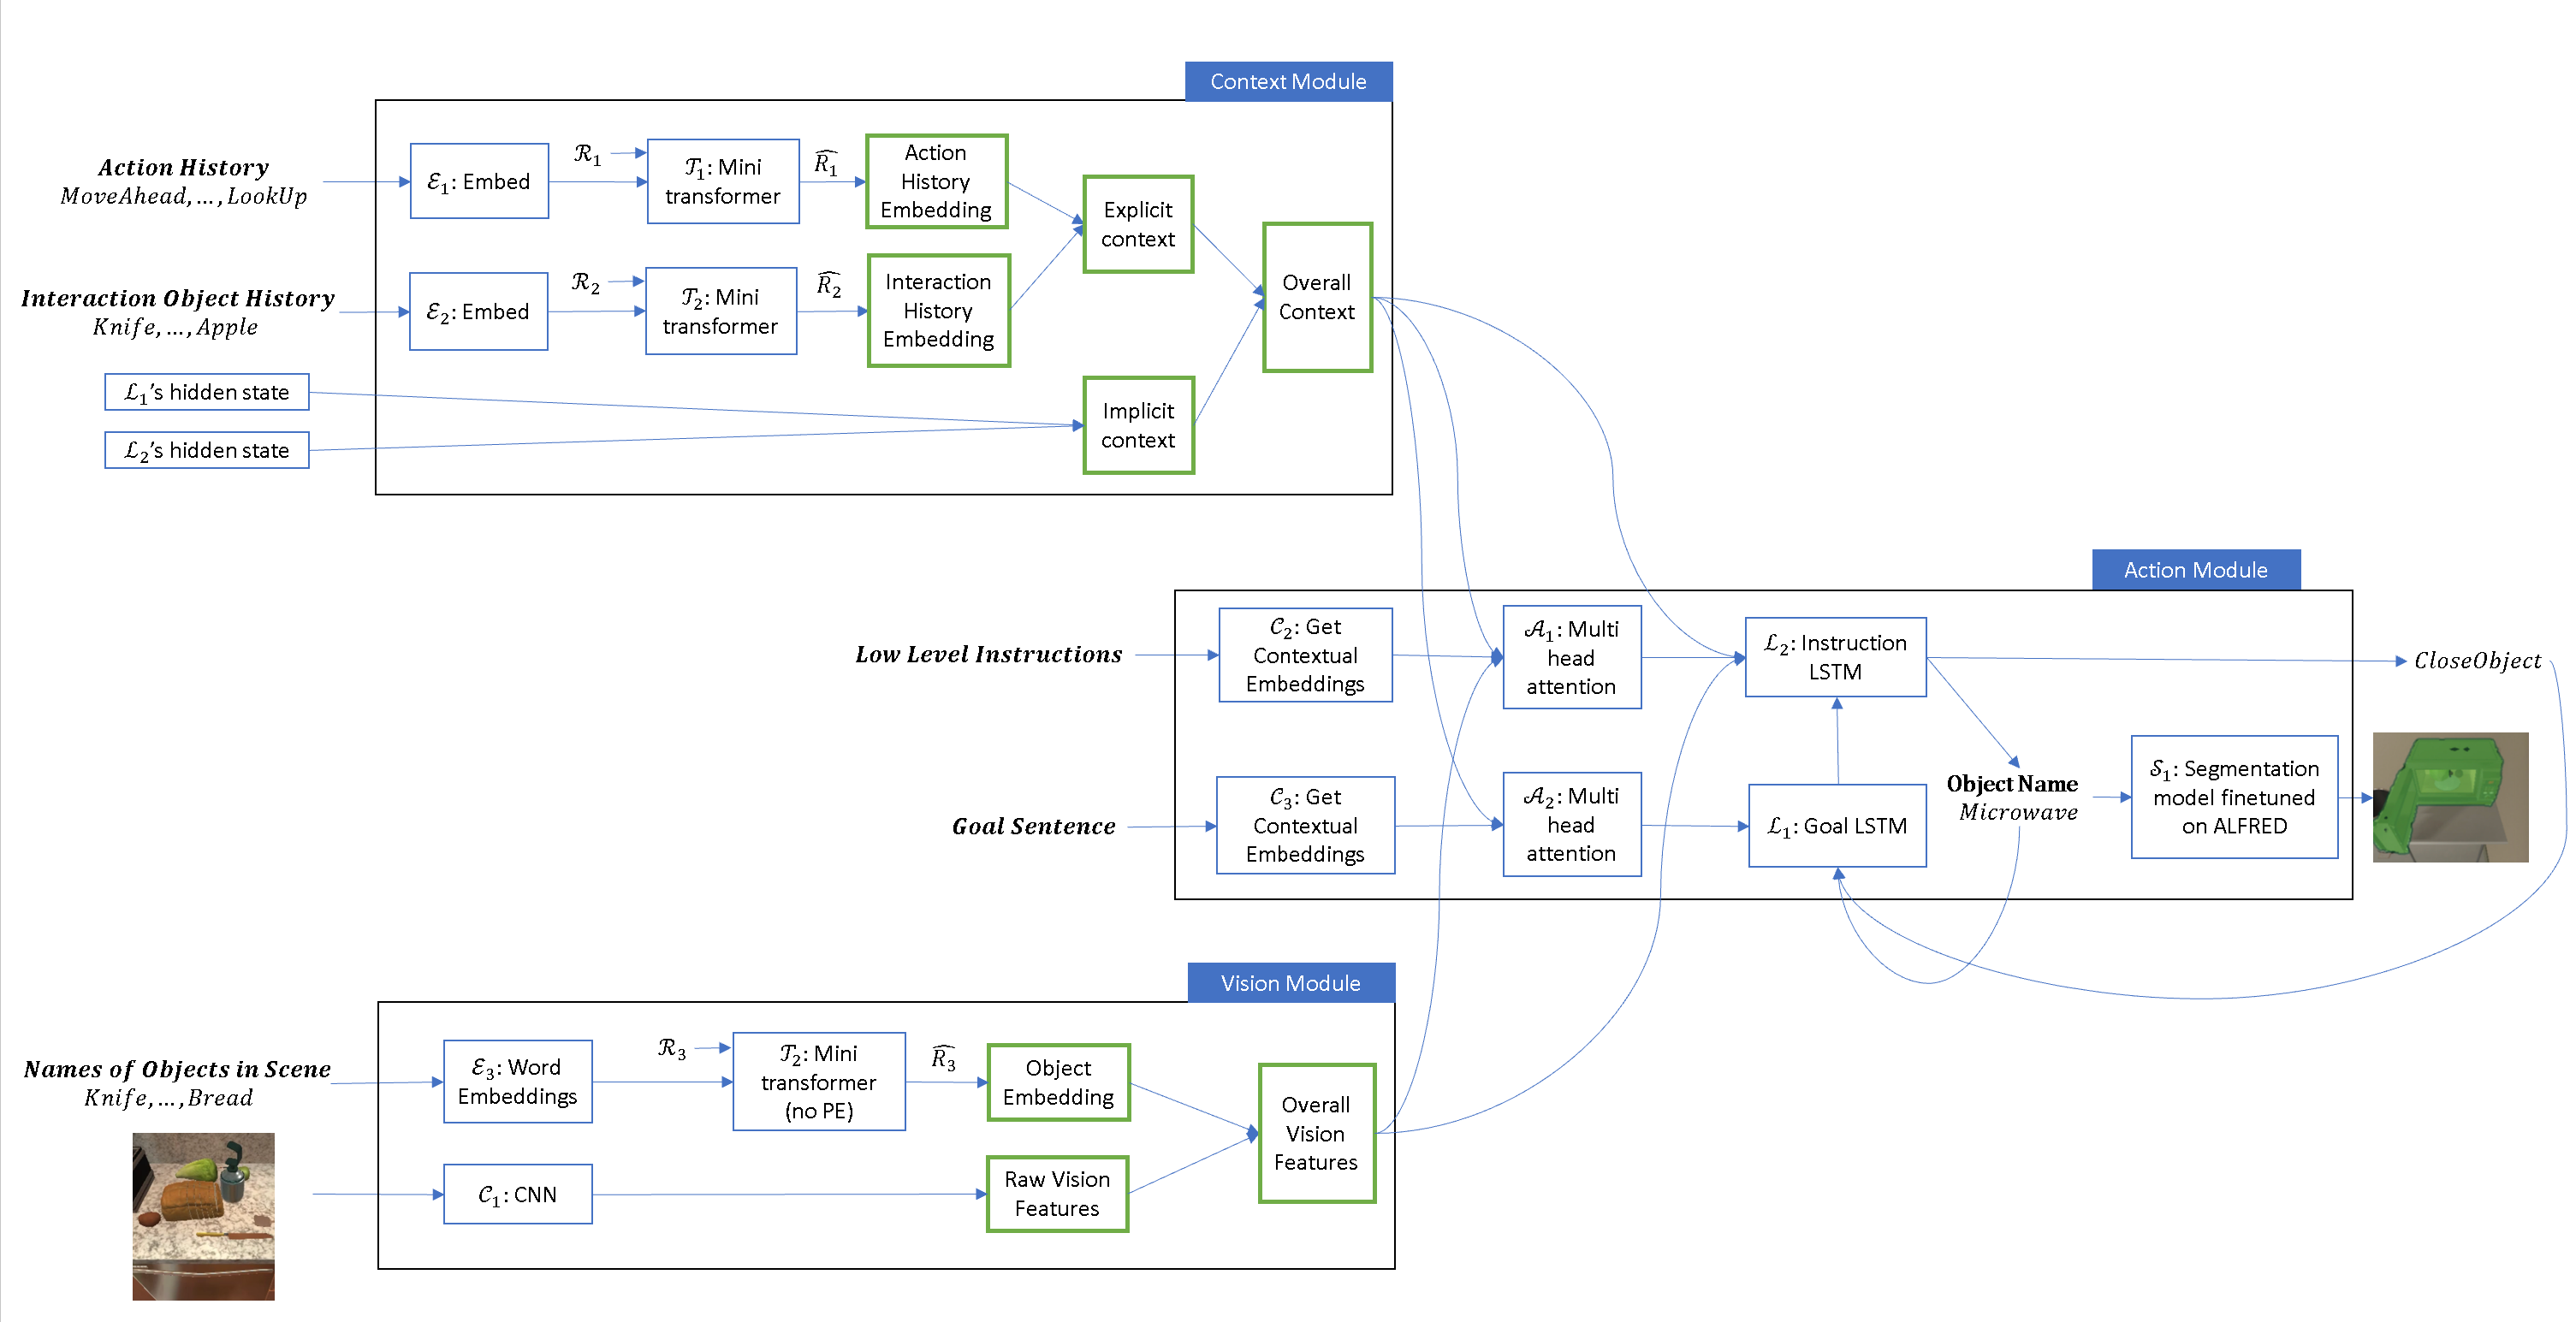
\includegraphics[width=\linewidth]{figures/tars_model.png}
    \caption{Our model consists of three novel modules as shown which are intended to provide better overall structure, stronger inductive biases, and more prior information to make it easier for each part of the model to learn. The model is explained in detail in \ref{sec:approach}}
    \label{fig:model}
\end{figure*}

\paragraph{Disentangling Explicit \& Implicit Context}
An important novel contribution of our method is to significantly lighten the load of each LSTM. As described in Section \ref{ssec:insights}, current architectures expect too much from their LSTMs. To this end, we provide some easily deducible history directly to our model, so the LSTM can only focus on learning a more latent and abstract form of context. This lets us essentially disentangle the explicit and implicit forms of context, which should make learning much simpler.

Specifically, we pass the last $k$ actions and the last $k'$ objects the agent interacted with as input.  As shown in the context module of Figure \ref{fig:model}, we use these two inputs to construct a representation of ``explicit context''. We combine this ``explicit context'' with the hidden states of our two LSTMs (which together form a representation of ``implicit context'') that form an overall context vector. We then use this overall context to perform attention over natural language instructions and goal as shown in Figure \ref{fig:model}. The intuition behind passing the last few actions and interaction objects is that any agent would need to keep track of its last few actions and interactions to have a good understanding of what its doing, so it makes more sense to just directly provide this history.

\paragraph{Grounding Language in Vision}
We propose a multimodal method to ground language in vision for the ALFRED task. Our insight is that it would be much harder for the model to align a raw visual representation (obtained from running a simple CNN on the input image) with a language representation because vision and language features are inherently different. If we can represent the image well using language, it would be much easier to align it with the instructions because both would be sequences of linguistic features. Our solution is to run an multi-label classifier on the input image and identify all objects in the image. Since these objects are just words, we pass them through an embedding layer followed by a transformer (without positional encodings because there is no inherent order) to get an overall representation (denoted ``object embedding'' in Figure \ref{fig:model}). As shown in Figure \ref{fig:model}, we use this object embedding and raw vision features to get ``overall vision features'', which are later used to attend over the natural language instructions as shown in the Action Module. We feel that language grounding would be much easier if we directly identify all objects in the image by their names because a) we are aligning language features with language features instead of vision features with language features, b) we are directly providing all objects in the scene as input, thereby significantly reducing the load of the CNN that outputs the ``raw vision features'' in Figure \ref{fig:model}. While we thought of this idea independently, we would like to point out that the idea of using object labels has been used in a previous ALFRED model \cite{Storks2021AreWT}, but in a different way. While \newcite{Storks2021AreWT} used this idea in a small module which was used to input additional features to the original baseline model \cite{shridhar2020alfred}, our idea has no dependence on the baseline model.

\paragraph{Two LSTMs}
Instead of using only one LSTM as in the baseline model \cite{shridhar2020alfred}, we use two different LSTMs: one to keep track of instructions, and another to keep track of the high level goal description as shown in the Action Module of Figure \ref{fig:model}. Having two LSTMs significantly reduces the responsibility of each because a clear disentanglement can be achieved between low level instruction following and high level goal completion. As shown in Figure \ref{fig:model}, the low level ``instruction LSTM'' is responsible for action and interaction object prediction based on overall context, vision features, and attended low level natural language instructions. The ``goal LSTM'' is then updated using the predicted action and object, and the natural language goal description is attended based on the overall context. Note that MOCA also uses two LSTMs as shown in Figure \ref{fig:moca_model}, but the LSTMs do not interact with each other, and they serve a very different purpose (keep track of perception and policy) than the two LSTMs in our model (keep track of overall goal and low level instructions).

\paragraph{Interaction Mask Prediction}
We follow MOCA's \cite{singh2020moca} approach of disentangling object class prediction and instance mask prediction. This makes the action predictor's job significantly easier because it only needs to identify the class of the object it needs to interact with (which often would be mentioned directly in natural language instructions) instead of identifying the object class, identifying the object in the current image, and then predicting a segmentation mask around the object. We plan to use MOCA's exact method of associating the actual object instance from the predicted object class using confidence and association-based measures.

\paragraph{Mini Transformer + Readout}
At various places in our model, we use a mini transformer to obtain one cumulative representation out of a given set of representations. We use the word ``mini'' to denote that we just intend to use 3-5 layers of the transformer instead of all 12.  As shown in Figure \ref{fig:model}, we use an additional input (denoted by $\mathcal{R}_1, \mathcal{R}_2, \mathcal{R}_3$) in all mini transformers. $\mathcal{R}_i$ is simply a learned vector added to each transformer, and serves the same role as a classification token does in BERT \cite{devlin2018bert}. The additional token is just used to \emph{readout} a vector (denoted by $\hat{\mathcal{R}_i}$) from the output of the transformer, which can then be used for downstream processing. This mini transformer + readout block is used whenever we want the input sequence to be processed with respect to other elements of the sequence. For example, it is important to process past actions with respect to each other so that the model knows exactly what the agent was trying to do in the past.

\section{Experimental Analysis (2 pages)}
While we unfortunately do not have full results on a trained model yet due to trying a fully novel model under strict compute limits, we discuss some of our key experiments in this section.

\subsection{Current State \& Future}
We have made tremendous progress on our model from where we started. We have run over 430 experiments, and our experiments' dashboard can be accessed at \url{https://wandb.ai/tars-alfred/group-tars-alfred}. While we were initially struggling to even make the model converge on a single demonstration and required fundamental changes in our idea, we have now successfully made our model converge on the entire training set, and have to just do more tuning to reduce over-fitting (which we do not have time and compute for). We want to note that while we have GCP/AWS credits remaining, we only have a quota of 1 GPU, which is why we cannot run experiments in parallel.

Our current model (36M parameters) is powerful enough to overfit the entire training set in just two epochs (see figure\ref{fig:overfit}, while the baseline model (45M parameters) takes 20 epochs and MOCA (70M parameters) takes 50 to produce the best model (not the most over-fitted one). We understand that speed of overfitting does not ultimately matter because we care about generalization, but overfitting so fast clearly with significantly fewer parameters shows that our model has the right inductive biases and capacity, and could potentially perform quite well with some more tuning in the future. Since our model is overfitting, our current validation performance is quite bad (i.e. validation loss is 10x more than training), but we feel that can be improved given time. Therefore, all results below only show training loss.

We now briefly present some ideas for the future. Currently we do not use any data augmentations, but we believe we can greatly improve performance with more data augmentations. For example, we could use color jitter on visual images, and cyclical translation (translate given sentence to a different language, and then tranlate back to English) on language data to generate more natural language sentences. As presented in class by some other ALFRED team, we feel that changing object poses and shuffling natural language instructions of different people can also be an effective augmentation strategy. It is important to note that we are not really ``stuck'' at any place currently, but just need more time and compute to make the model generalize well.

\begin{figure}
    \centering
    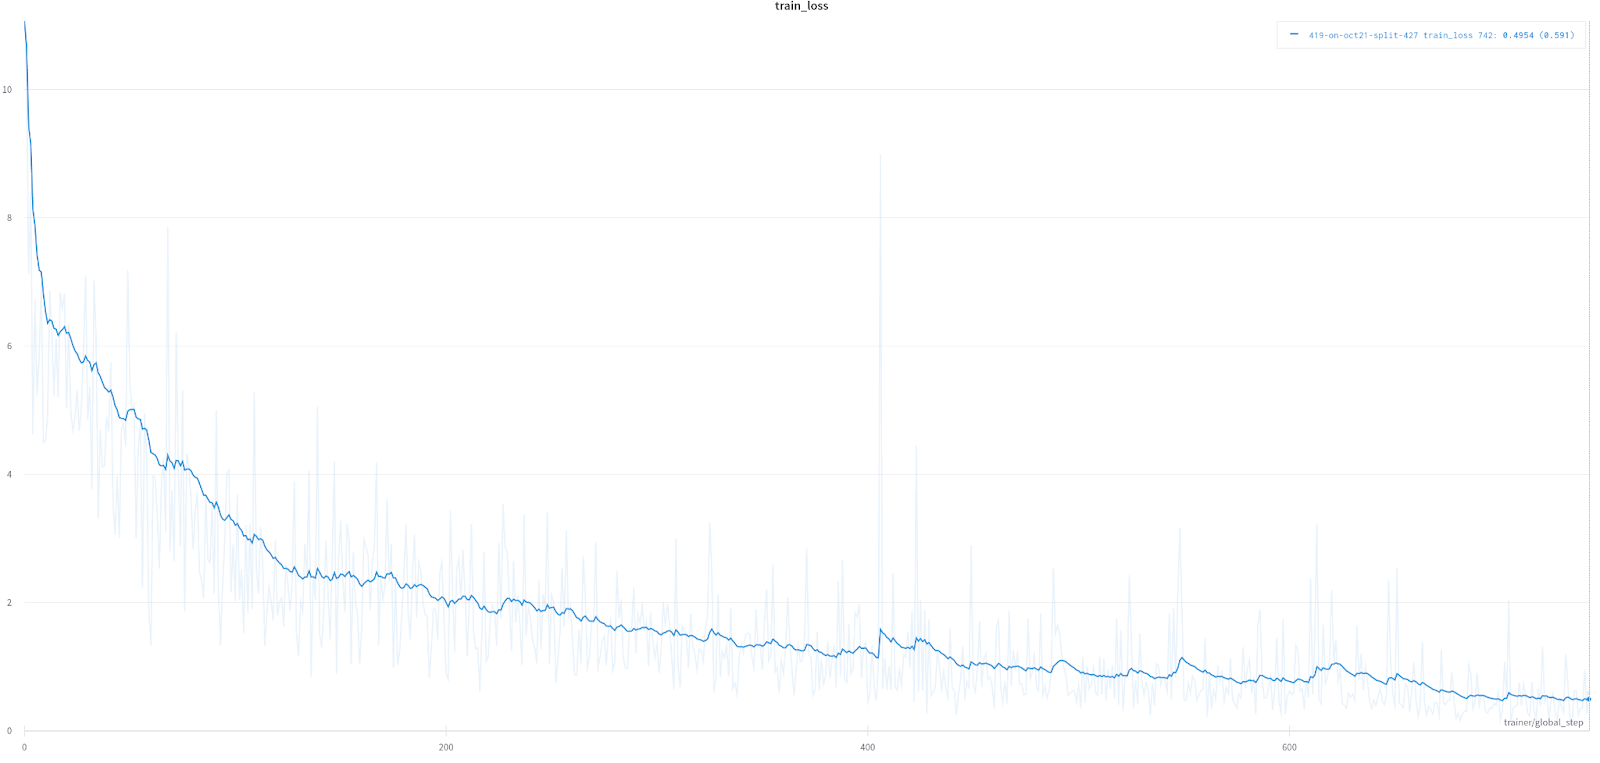
\includegraphics[scale=0.13]{figures/loss_curve.png}
    \caption{This graph shows the training loss over the full training split for almost two epochs. Clearly, the loss goes quite close to zero. Full experiment is \href{https://wandb.ai/tars-alfred/group-tars-alfred/runs/21ktm5uf}{here}.}
    \label{fig:overfit}
\end{figure}

\subsection{Key Experimental Findings}

In this section, we discuss some key experimental findings, and provide some more experimental findings in Appendix Section \ref{ssec:add-exp}.

\textbf{Small Splits.} We could not afford training on the whole training split often to test our model because just one epoch costed us 16 hours. So, we created many versions of the small splits to quickly debug and test the model capacity at different layers. Specifically, we created a split with just a single demonstration to see if we could at least overfit that, a split with 20 demonstrations, and a split with all pick and place demonstrations so we could test the overall capacity of the model and test big changes on a relatively larger split. 

\textbf{Thorough Tuning.} Since our model had so many different components and parts, we had to spent significant time optimizing and tuning our model to extract best performance. Figure \ref{fig:hp-tuning-comp} shows the effect of good tuning on the model: it helped our model overfit the small split about 100 epochs faster. Specifically, we observed that adding layer normalization layers, using Adam optimizer (instead of SGD), having a higher batch size (16) compared to baseline model (8), and initializing convolution, multihead attention, linear transformers, embeddings, and LSTM with the same settings of Kaiming normal method significantly helped the model. In particular, we want to stress that most packages have different initializations for every layer, but we found out that using the same initialization method across layers significantly speeded up learning in our case.

\begin{figure}
    \centering
    \begin{subfigure}[b]{0.5\textwidth}
    \centering
    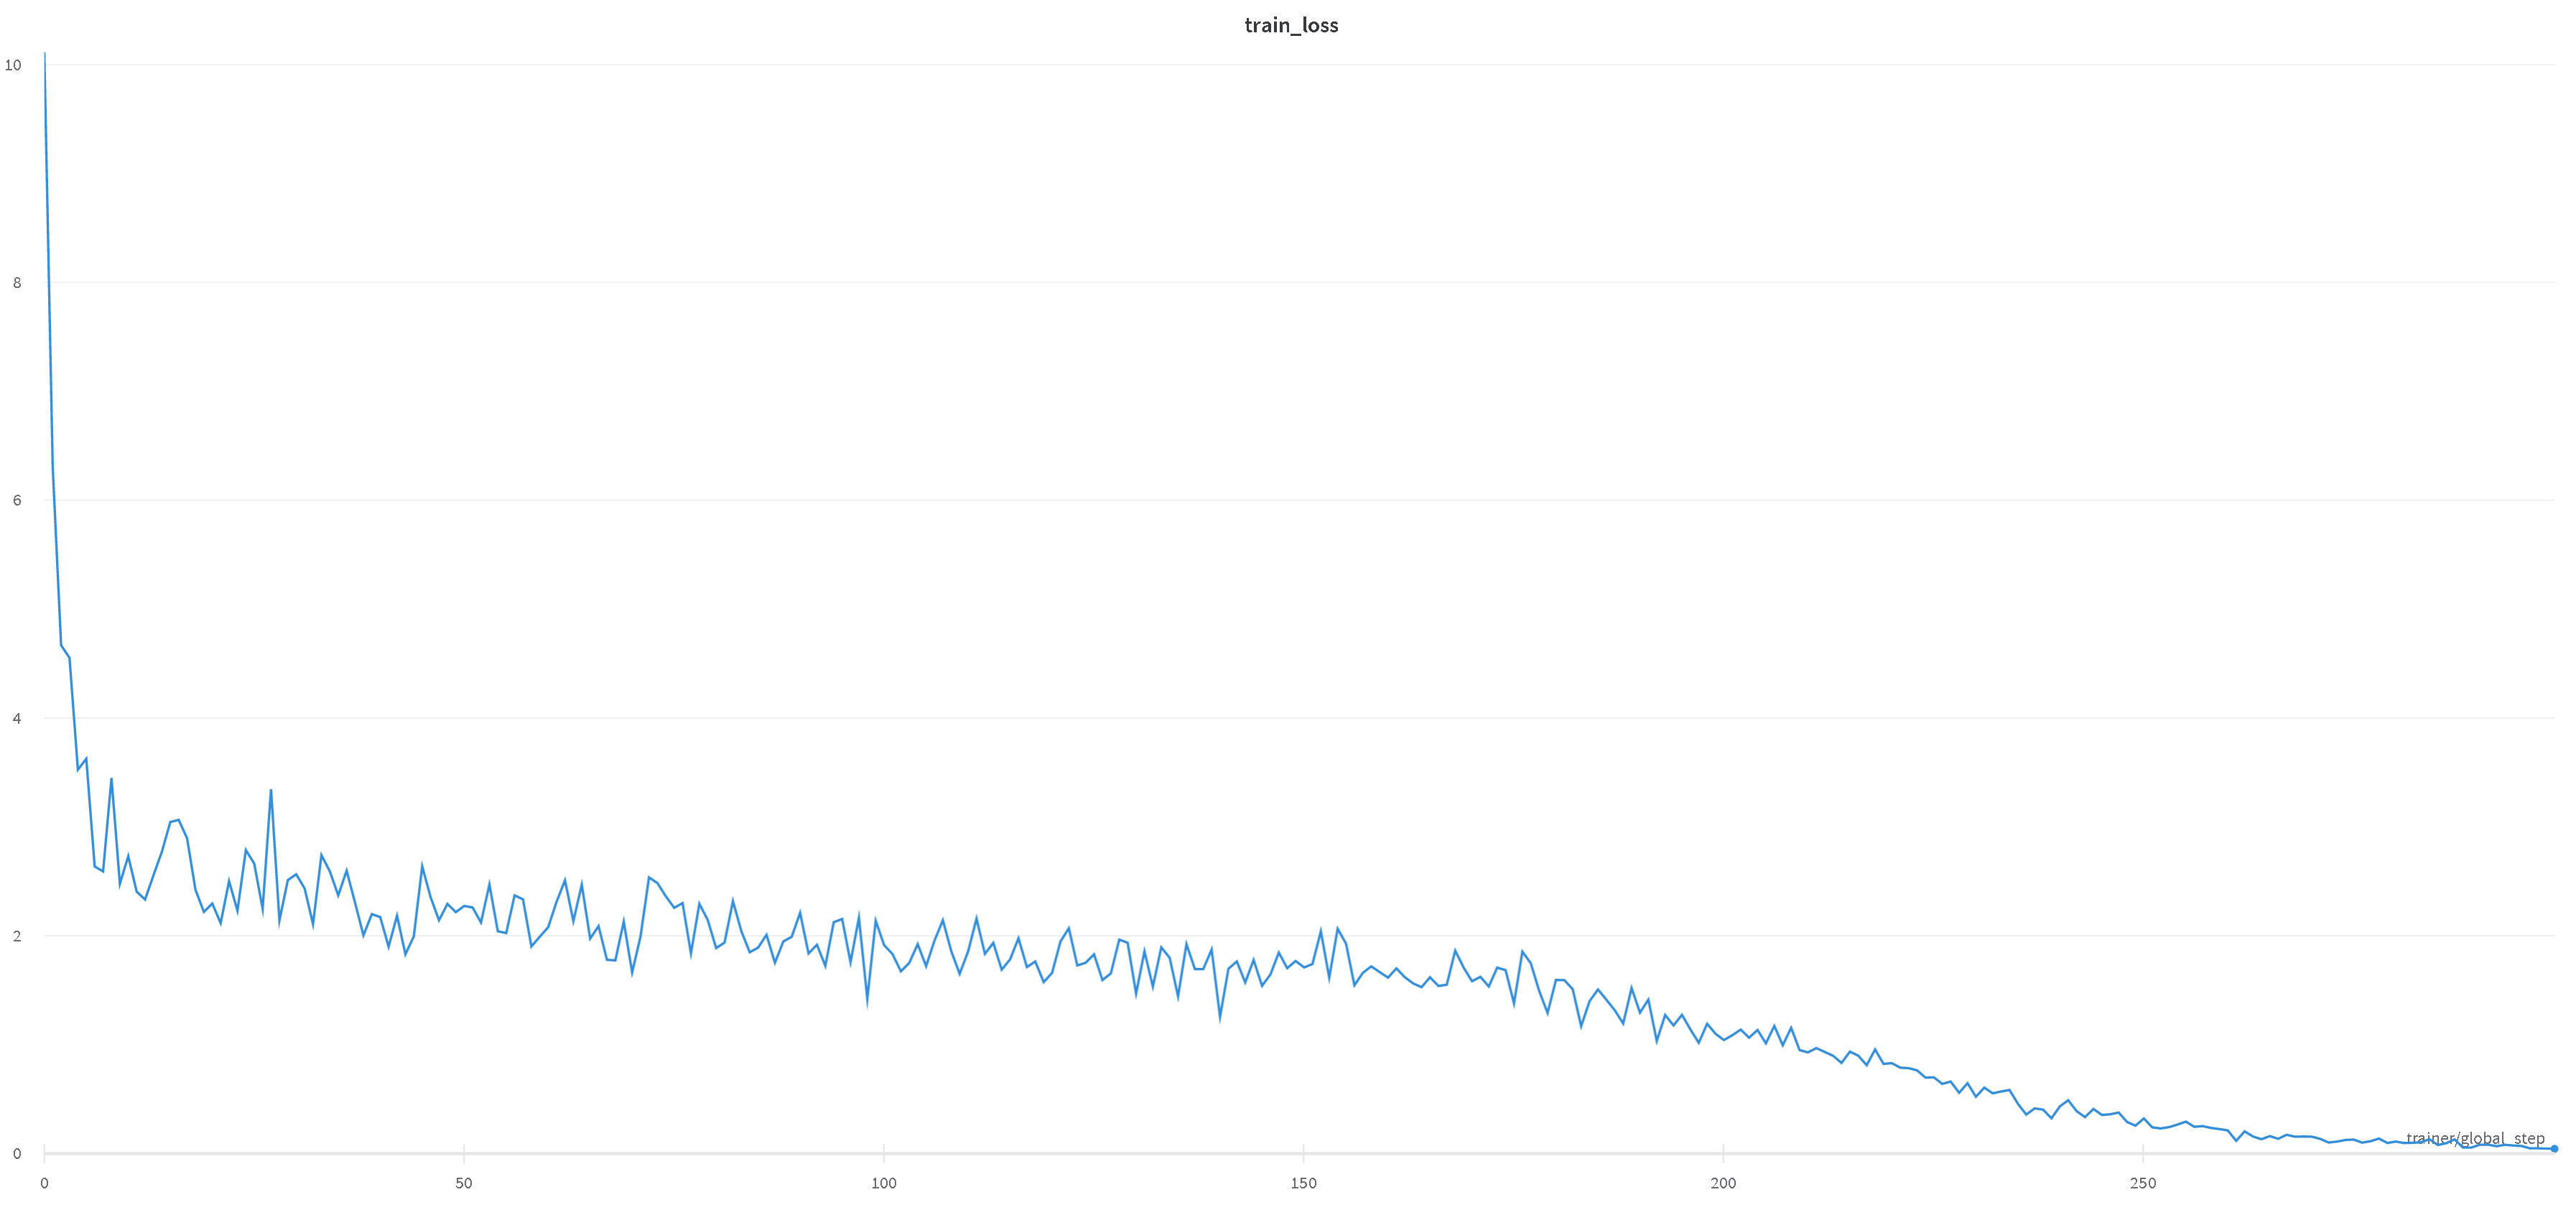
\includegraphics[scale=0.2]{figures/initial_loss_one_task.png}
    \caption{}
    \end{subfigure}
    \hfill
    \begin{subfigure}[b]{0.5\textwidth}
    \centering
    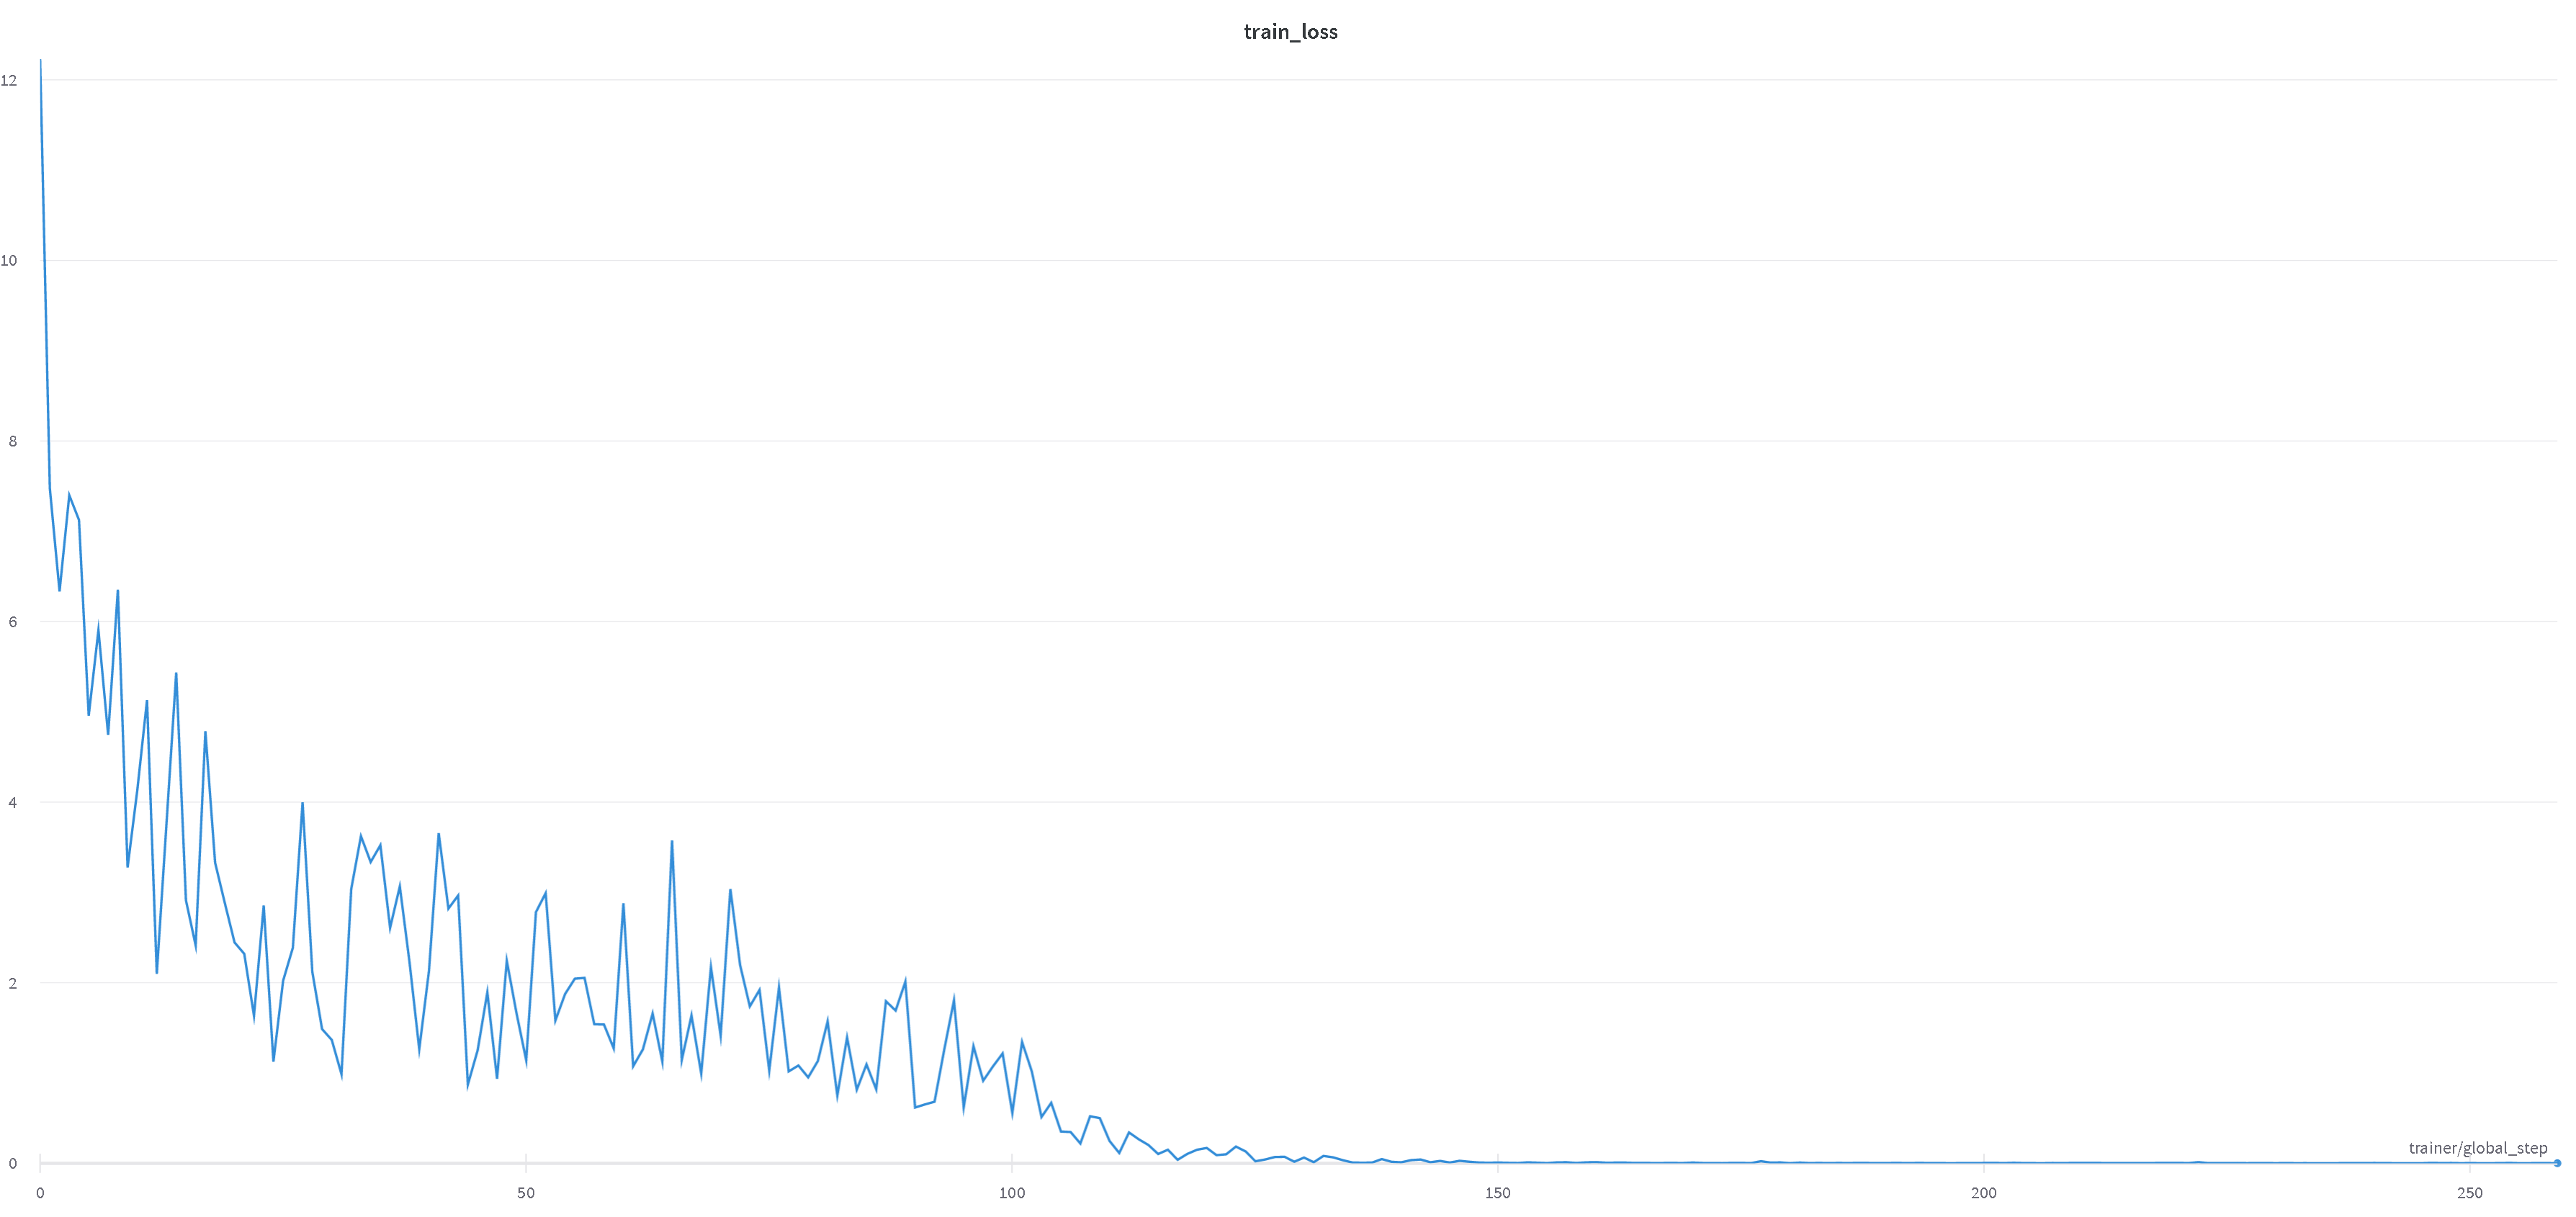
\includegraphics[scale=0.2]{figures/hp_tuned_loss_one_task.png}
    \caption{}
    \end{subfigure}
    \caption{The top figure shows the training loss of our model with little tuning on a single demonstration, while the bottom one shows the loss of a well tuned model which overfits the demonstration about 100 epochs faster.}
    \label{fig:hp-tuning-comp}
\end{figure}

\textbf{Vision Module Changes.} Initially, to get raw vision features in Figure \ref{fig:model}, we were simply running a ResNet18 with a liner layer on top and tuning the last 25\% of the model layers (rest were frozen). However, we noticed that the baseline model did things differently to keep the spatial structure somewhat intact. The baseline model used the output of last convolution layer in ResNet, passed it through several 1x1 convolution layers before flattening it. We tried to use the same idea in our model, and noticed an instant boost in speed of convergence on small splits as shown in Figure \ref{fig:baseline-vision}. Also, note that we did not have enough parallel compute to train a multi label classifier well on images (though we tried with several models), so we chose remove ``object embedding'' (see Figure \ref{fig:model}) from our final model, and just used raw vision features.

\begin{figure}
    \centering
    \begin{subfigure}[b]{0.5\textwidth}
    \centering
    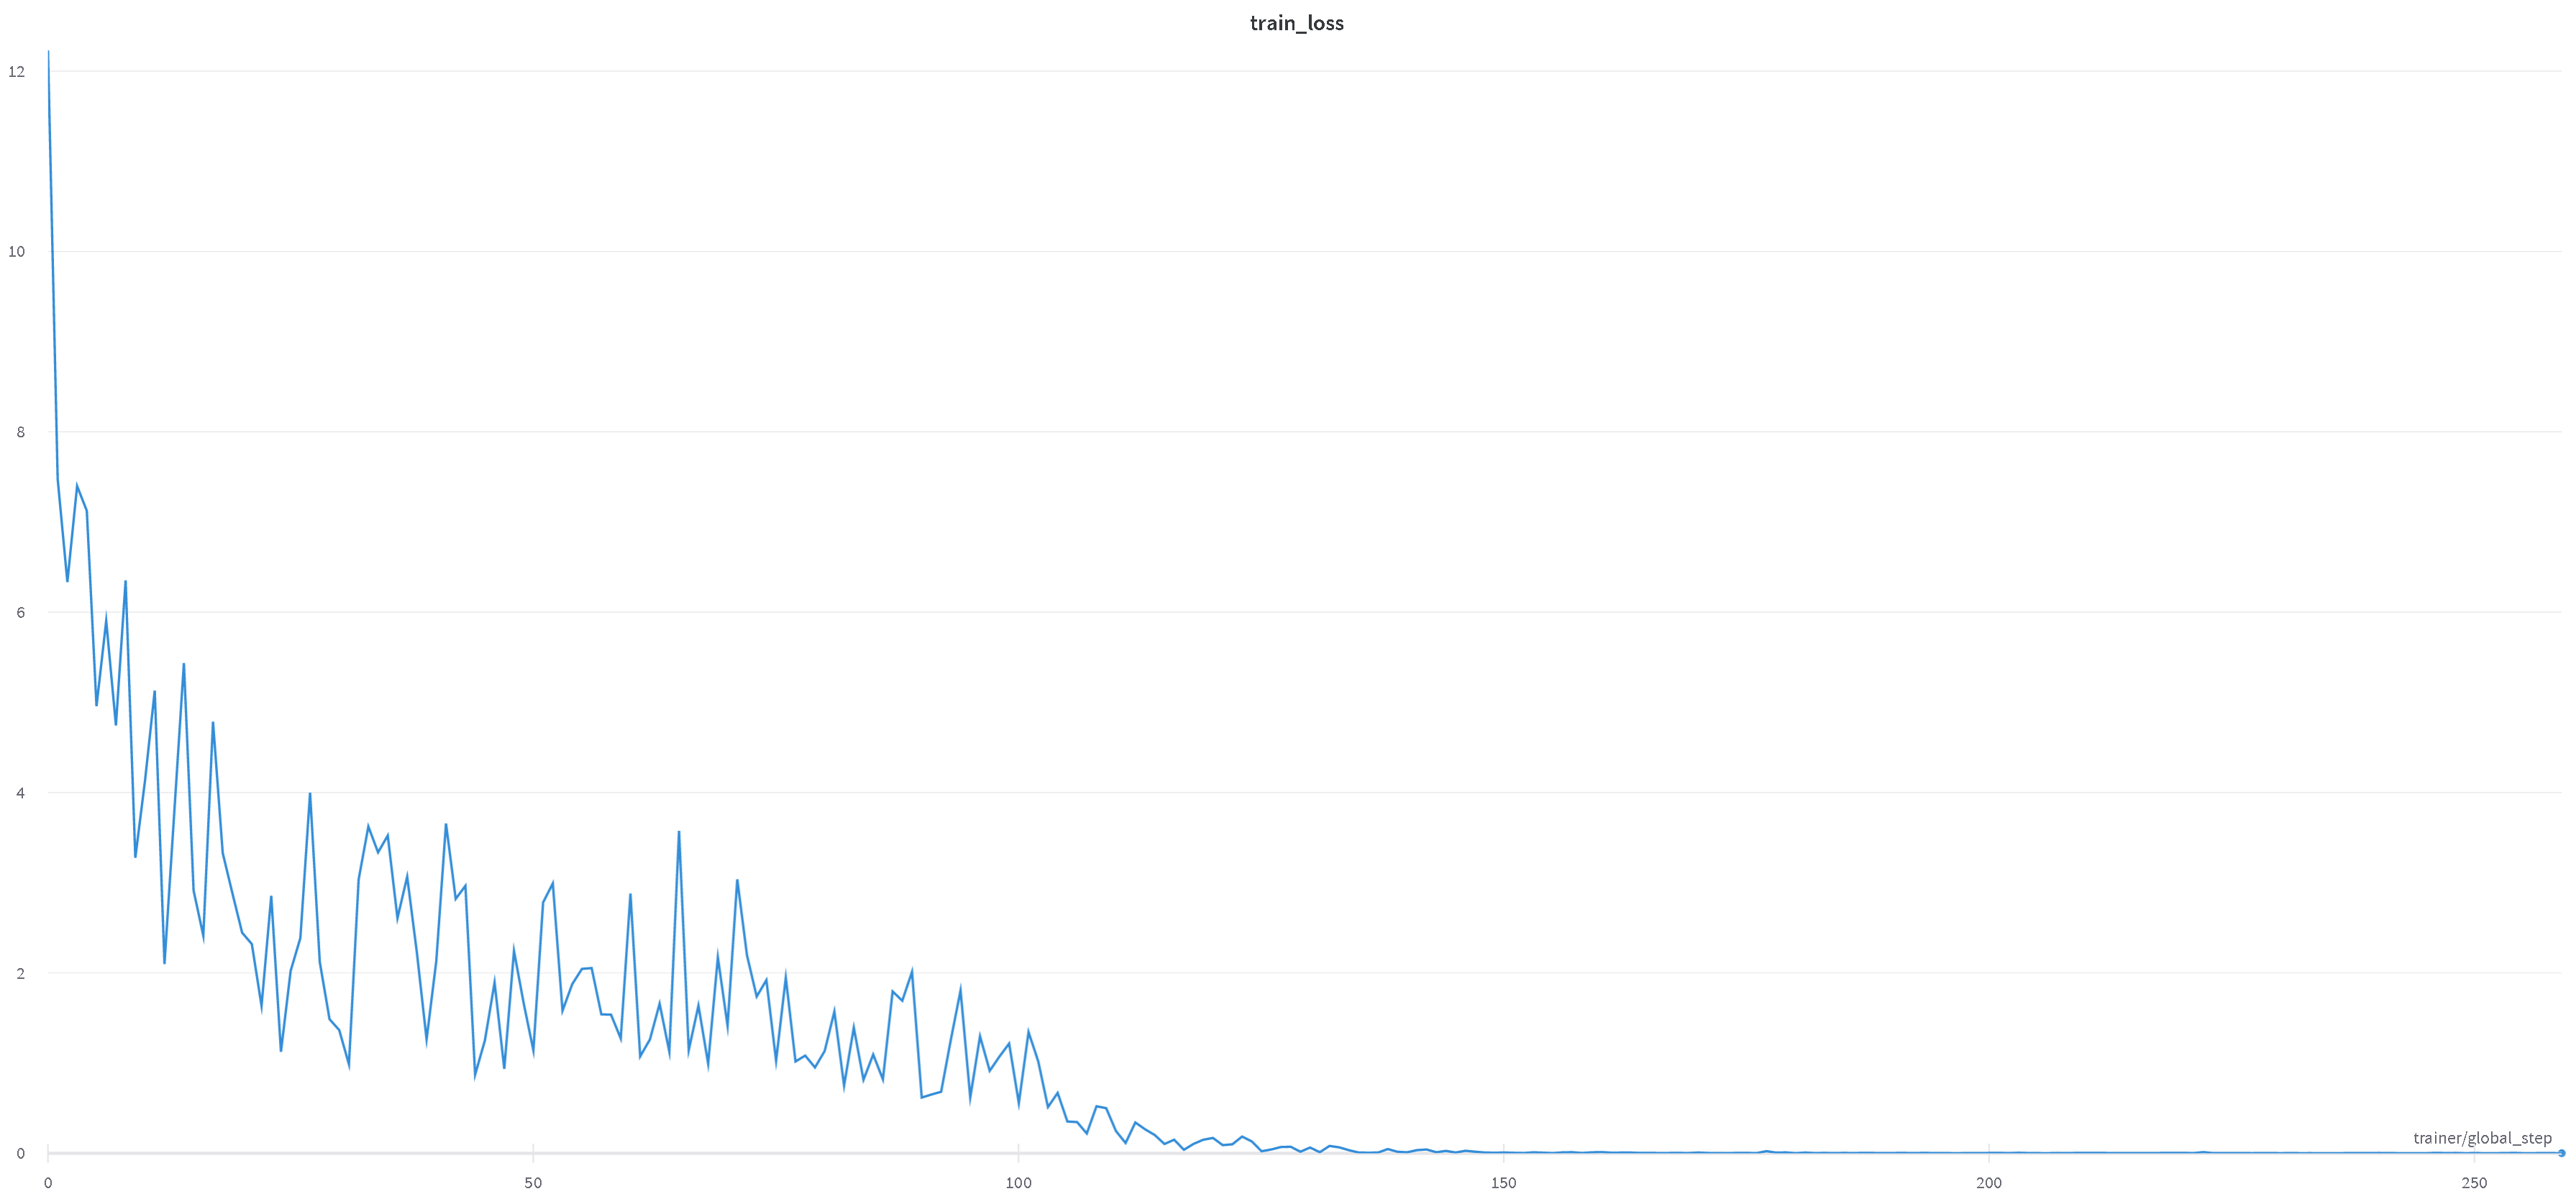
\includegraphics[scale=0.2]{figures/adam_loss.png}
    \caption{}
    \end{subfigure}
    \hfill
    \begin{subfigure}[b]{0.5\textwidth}
    \centering
    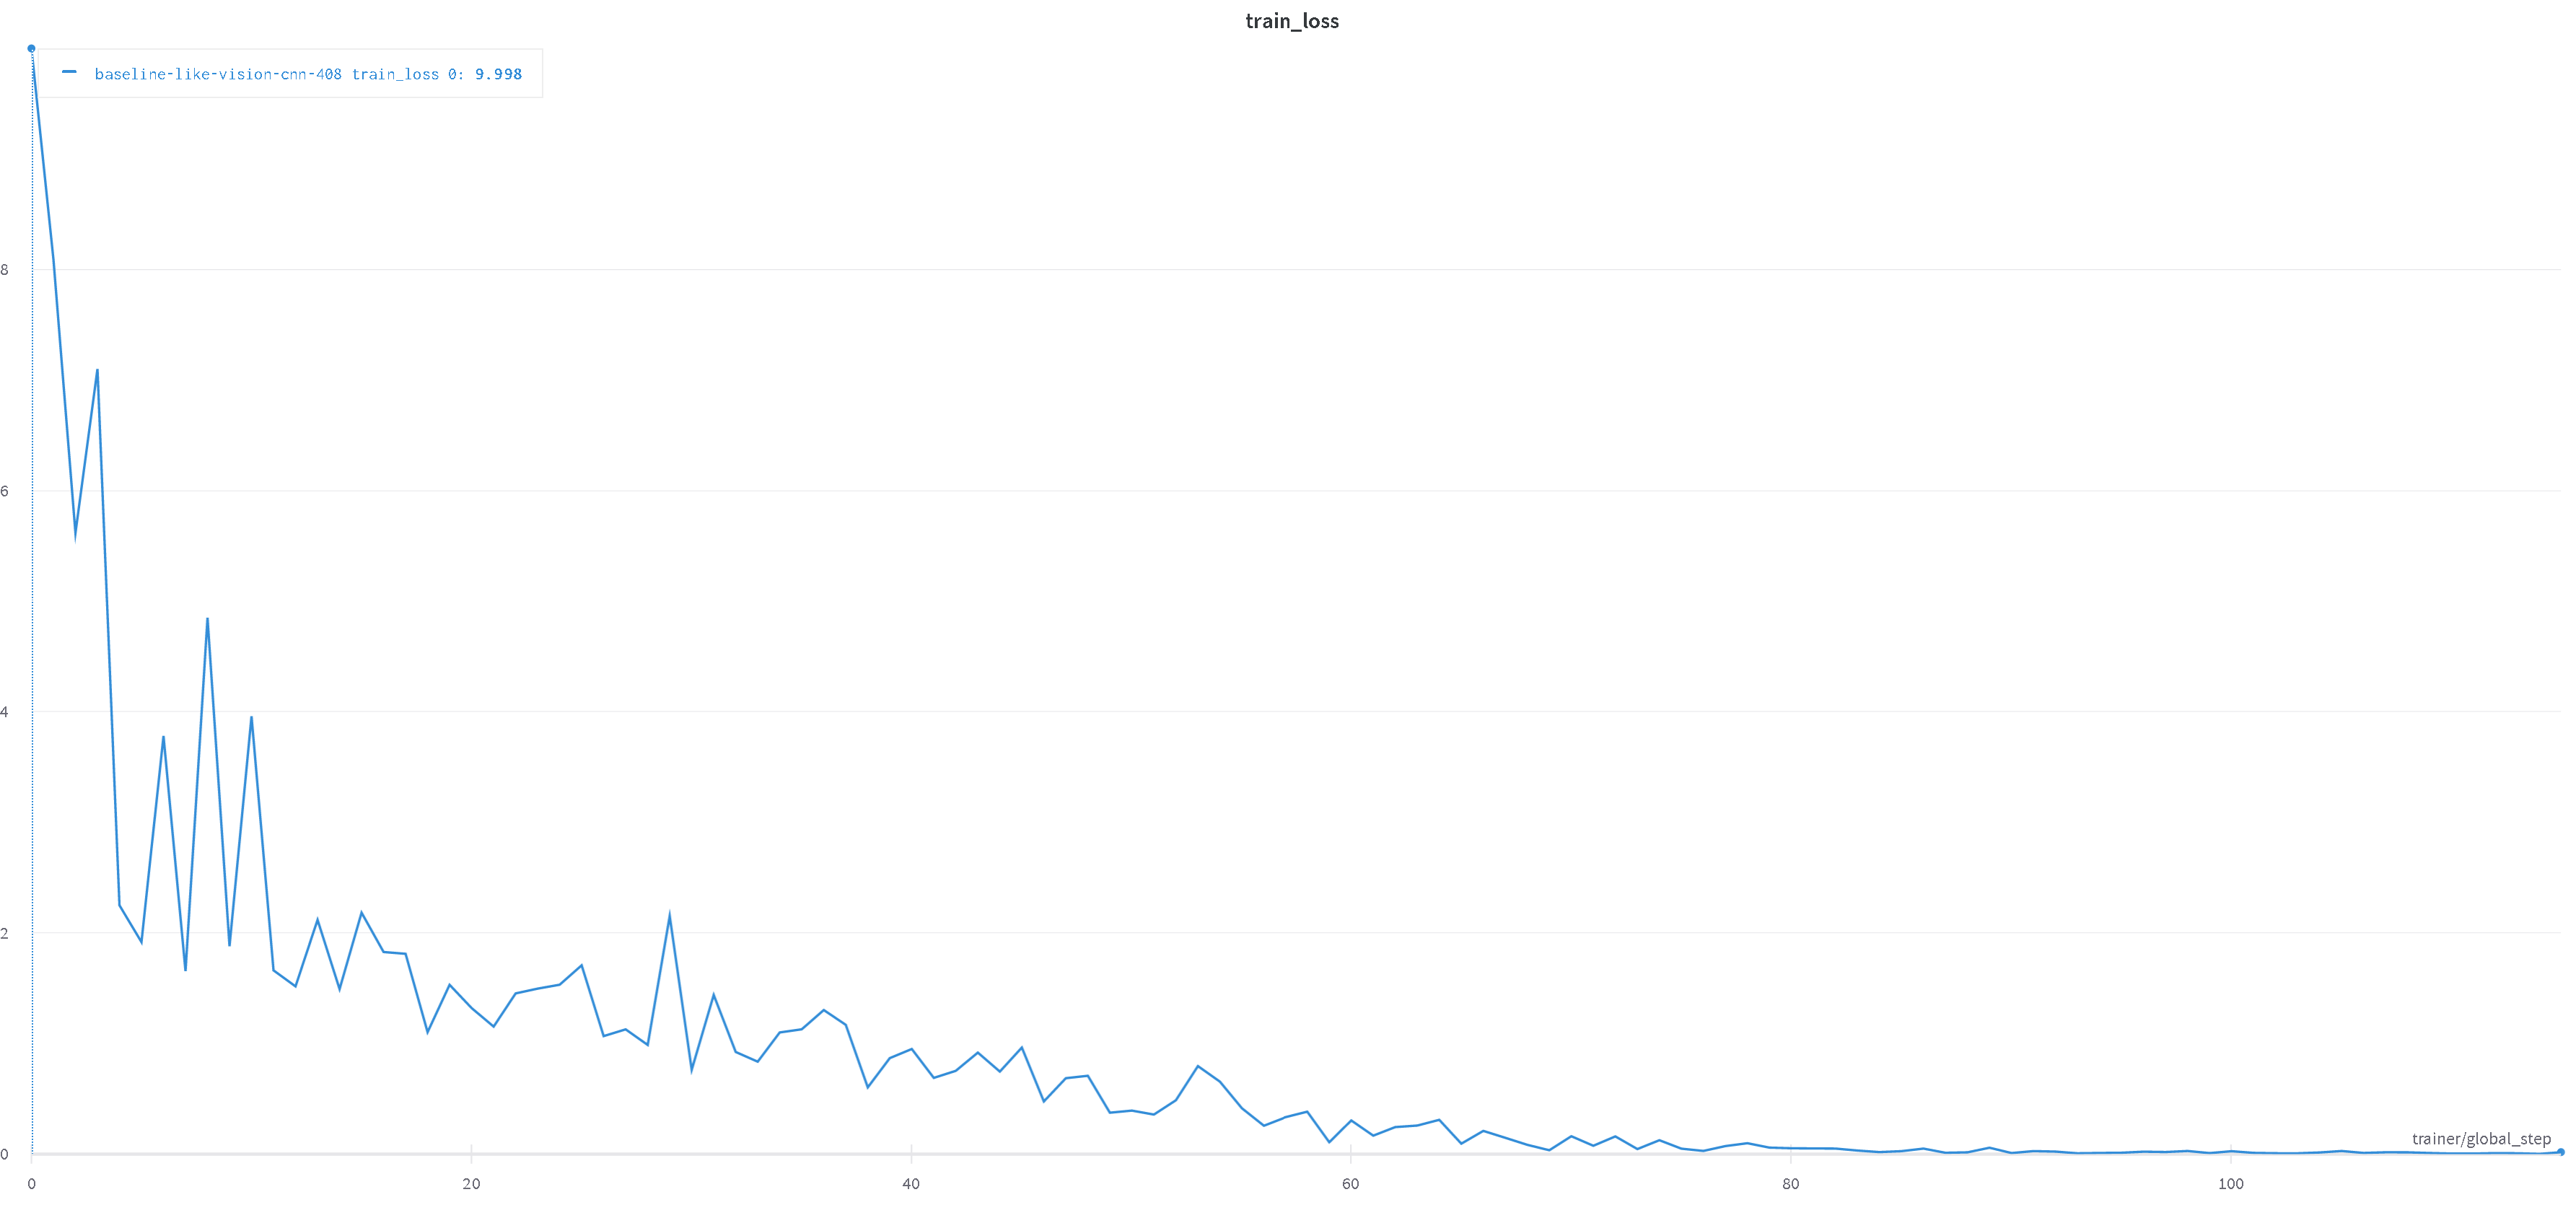
\includegraphics[scale=0.2]{figures/baseline_vision_loss.png}
    \caption{}
    \end{subfigure}
    \caption{The top figure shows the training loss (on 20 tasks) of our model when using visual features of just a ResNet18, while the bottom one shows the loss of the model when extracting visual features like the baseline model \cite{shridhar2020alfred}. Clearly, the latter overfits the about 50 epochs faster.}
    \label{fig:baseline-vision}
\end{figure}

\textbf{Separating Action and Object LSTMs.} We noticed that the action prediction loss was reducing at a much slower rate than the object prediction loss. Originally, action and object was predicted by two heads on top of the instruction LSTM in Figure \ref{fig:model}, and we hypothesized that it may be better to have two LSTMs instead of a common instruction LSTM: one for predicting actions, and another for predicting objects. Having two separate LSTMs also allowed us to condition the object LSTM on the predicted action, so predicting objects becomes easier. While we don't include plots here due to space limits, our experiments showed a minor improvement when using two separate LSTMs, so we stuck to this design for future runs.

\textbf{Other Architectural Changes.} We also tried several more architectural changes to improve information flow in the network. For example, we tried different transformer based methods to get contextual embeddings. We also explicitly passed the action history to the instruction LSTM in addition to the context vector for better gradient flow. We also noticed that pretraining the transformers in the context module did not really help much. We also tried passing the predicted action and object to the goal LSTM, so its easier to keep track of where the agent is in achieving the overall goal. Most of these changes had minor improvements to the speed of convergence.

\textbf{Total Parameters.} When we started training our best models optimized on small splits on larger splits, we noticed that the variance in loss was high and loss was not decreasing. We analyzed MOCA and the baseline model to find out the reasons, and realized that our model was using only 27M parameters, while MOCA was using 70M, and baseline was using 45M parameters. When we simply increased parameters in our model to 55M, we started finding that our model was able to significantly overfit the larger sets (i.e. sub-zero training loss, high validation loss). As said before, some further experiments also showed that our model was able to overfit the training set even with 36M parameters, which is smaller than all previously proposed models.


% \subsection{Qualitative Analysis and Examples}
% This section should likely contain a table of examples demonstrating how the current approach succeeds/fails.

% Please use 
\bibliographystyle{acl_natbib}
\bibliography{references}

\appendix
\section{Appendix}

\subsection{Dataset Analysis}
In this section, we present a subset of the analysis we performed. We encourage the reader to see the Jupyter notebook stored in the \emph{Analysis} folder for full list of figures pertaining to the analysis since this report only includes a subset.

\paragraph{Dataset Statistics}
Table \ref{tab:dataset-means} shows average values for the quantitative metrics measured on ALFRED: importantly, averages are fairly consistent across splits. 

\begin{table}[H]
\small
\resizebox{\linewidth}{!}{%
\begin{tabular}{@{}llll@{}}
\toprule
                                     & \textbf{Train} & \textbf{Valid (seen)} & \textbf{Valid (unseen)} \\ \midrule
{Steps per directive}                       & 6.68           & 6.64                 & 6.27                   \\
{Tokens per step}                   & 12.39          & 12.18                & 12.63                  \\
{Task desc. tokens}                  & 10.02          & 10.09                & 10.04                  \\
{Images}                      & 286.75         & 287.24               & 277.72                 \\
{Actions}                     & 49.78          & 50.12                & 46.98                  \\
{Images per action}               & 6.08           & 6.02                 & 6.12                   \\
{Actions per step}                & 7.6            & 7.72                 & 7.72                   \\
{Nav-interact ratio}                & 9.19           & 9.25                 & 8.13                   \\
{Total objects}              & 33.2           & 32.84                & 38.44                  \\
{Mask coverage} & 0.17           & 0.17                 & 0.15                   \\
{Step-object coverage}    & 0.86           & 0.85                 & 0.88                   \\ \bottomrule
\end{tabular}%
}
\caption{Average values of various quantitative aspects of ALFRED by split. See below for definitions.}
\label{tab:dataset-means}
\end{table}

In Figure \ref{fig:task-type}, we see that ALFRED contains a roughly equal number of demonstrations for each type of task, and for the most part, a roughly equal proportion for each split. The validation data, especially the unseen portion, does have relatively less ``Pick Two \& Place'' tasks than the training data. Additionally, the unseen portion has a significantly higher proportion of ``Examine in Light'' tasks than the other splits.

Furthermore, Figure \ref{fig:action-freq} shows the frequency of the 12 different actions (5 navigation actions + 7 interaction actions). Note that all splits have fairly equal frequency for all actions and 60\% of actions are ``move ahead'' actions.

The navigation-interaction ratio indicates that for every interaction action in a demonstration, there are roughly 9 navigation actions. The mask coverage indicates that on average, the ground-truth interaction mask covers a rather small (15-17\%) proportion of the image. The step-object coverage of nearly 1 indicates that for almost all interactions, the name of the object of interest is mentioned in the corresponding language directive. By manually inspecting examples with low interaction step coverage, we find that the object's name are usually substituted with a synonym (e.g.``rag" for ``cloth" and ``scoop" for ``ladle").

\paragraph{Description of fields in Table \ref{tab:dataset-means}}
\begin{enumerate}
    \item Steps per directive: number of steps in each language directive
    \item Tokens per step: number of words in each directive step
    \item Task description tokens: number of words in directive task description
    \item Images: number of images per demonstration
    \item Actions: number of actions per demonstration
    \item Images per action: number of images divided by number of actions per demonstration
    \item Actions per step: number of actions divided by number of directive steps per demonstration
    \item Nav-interact ratio: number of navigation actions divided by number of interaction actions per demonstration
    \item Total objects: number of total objects in a scene per demonstration
    \item Mask coverage: proportion of the image that is covered by the interaction mask per demonstration
    \item Step-object coverage: proportion of interaction actions whose object of interest is mentioned in the step-by-step instructions, averaged over all interaction actions and language directives in the demonstration
\end{enumerate}



\begin{figure}[H]
\centering
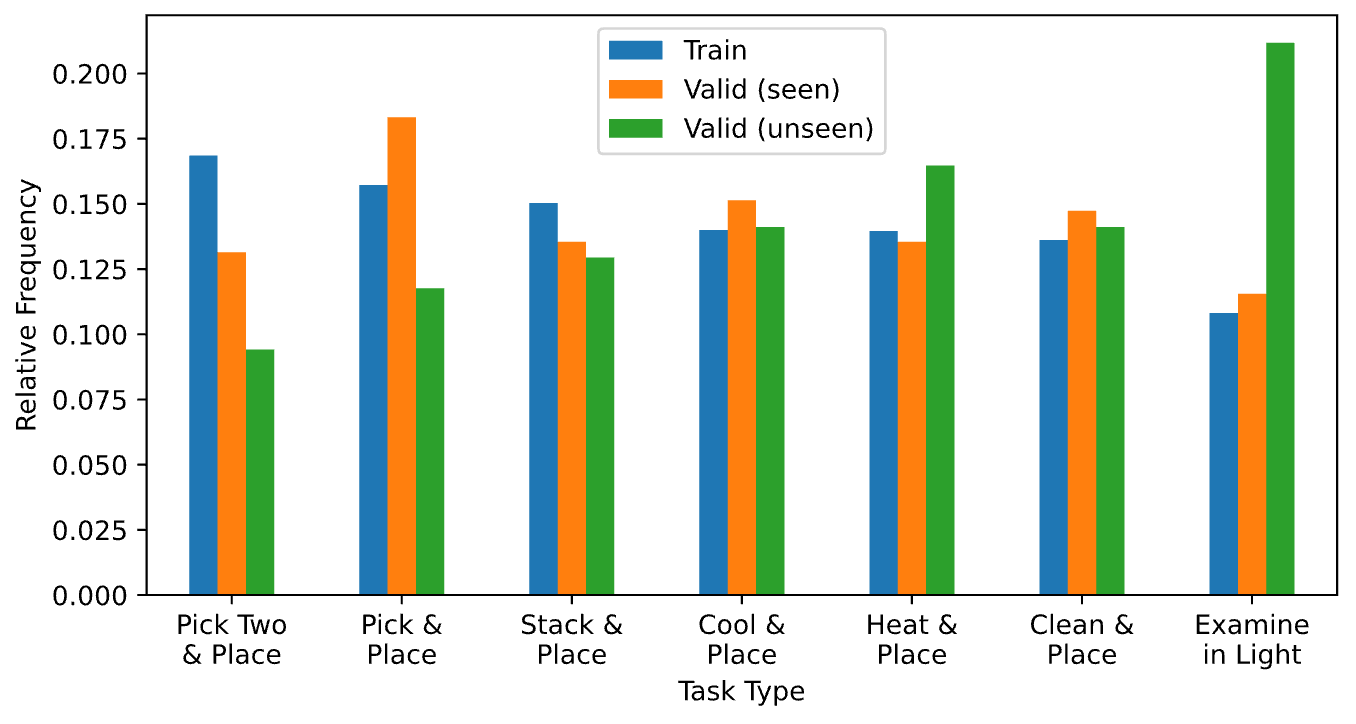
\includegraphics[scale=0.33]{figures/task_type_freqs.png}
\caption{Relative frequency of each task type by split.}
\label{fig:task-type}
\end{figure}

\begin{figure}[H]
\centering
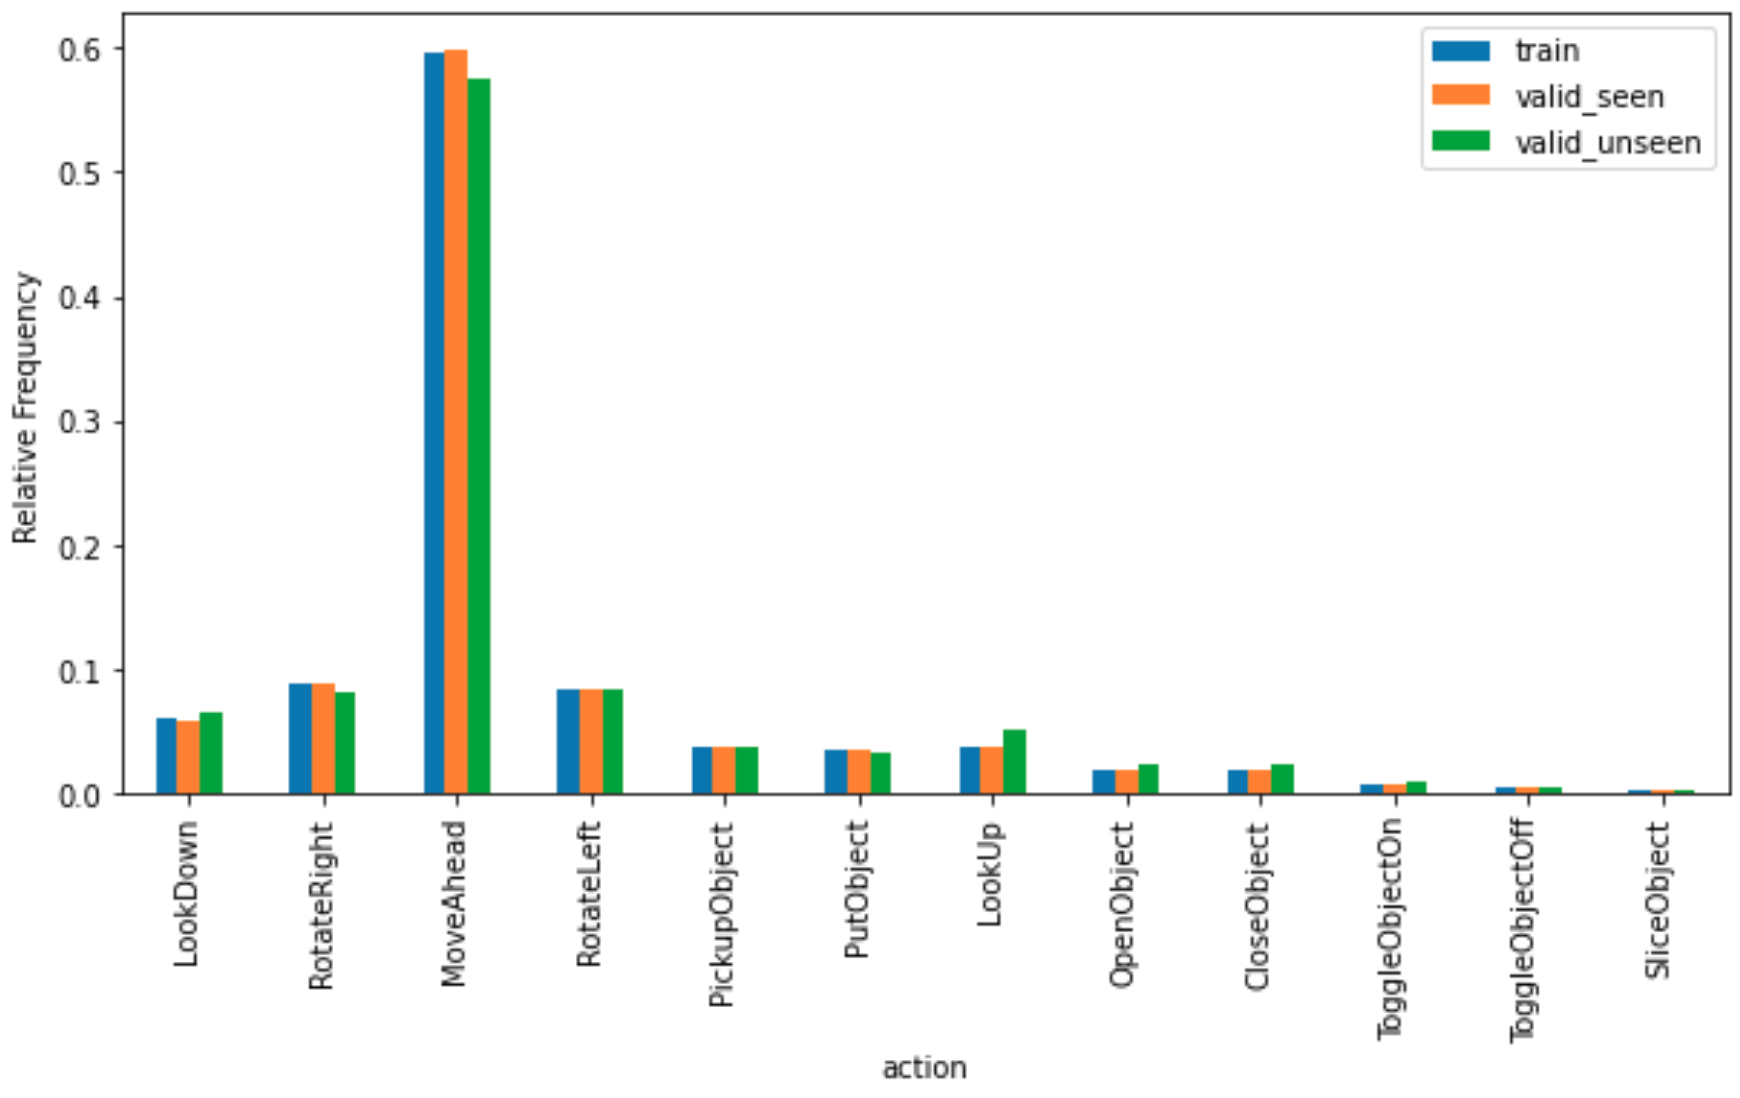
\includegraphics[scale=0.13]{figures/action_freq.png}
\caption{Relative frequency of each action type by split.}
\label{fig:action-freq}
\end{figure}

\begin{figure}[H]
\centering
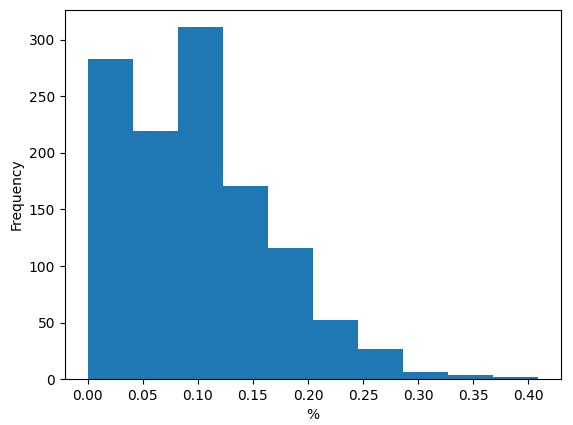
\includegraphics[scale=0.33]{figures/objects_vs_instructions.png}
\caption{Percentage of objects referred to in instructions compared to objects in the scene}
\label{fig:object-vs-instruction}
\end{figure}

\paragraph{Textual Analysis}
For textual analysis, we first analyzed how many objects present in the scene are directly referred to in the step-by-step instructions. The results are plotted in a histogram in Figure \ref{fig:object-vs-instruction}, which reveals that much less than 40\% of objects in the scene are actually referred to in the instructions. 

We additionally identified out of vocabulary (OOV) words in the training and validation set using a vocabulary of 685k words defined by spaCy. We found that less than 0.002\% of all words were OOV in any split, indicating the dataset is already quite clean. Most of the OOV words were just misspelled (eg: "stovve"), indicating that it would be important to preprocess text using a simple spell checker before using it for downstream tasks.

We also found the top few synonyms used to describe objects in the dataset. This was performed by comparing the similarity of word vectors of all objects in the dataset with all common nouns identified in all task descriptions. The complete results are in the Jupyter notebook, but a few results are shown in Table \ref{tab:synonynms}. This reveals that our model will need to be robust enough to recognize synonyms of different words in order to be successful. 

\begin{table}[H]
\small
\begin{tabular}{@{}ll@{}}
\toprule
Object Name & Synonyms used in task descriptions  \\ \midrule
Coffee Machine & Espresso Machine, Beverage Machine \\
Chair & Couch Chair, Sofa Chair \\
CD   & DVD \\
Side Table & Corner Table \\
Butter Knife & Bread knife \\
Ottomon & Loveseat, Recliner \\
Fridge & Kitchen Fridge, Refrigerator \\
Poster & Wall Photo, Picture \\
Safe & Safety Box \\ 
Soap Bottle & Lotion Bottle
\end{tabular}

\caption{Synonyms (i.e. closest words in embedding space) used in task descriptions of some objects in the dataset}
\label{tab:synonynms}
\end{table}




\paragraph{Visual Analysis}
% image sizes, which preprocessing techniques will help, visual quality
Due to compute constraints, most visual analysis was performed qualitatively by inspecting visual quality of different types of images. Figure \ref{fig:sample_ims} shows some sample RGB, depth and instance segmentation images. All images retrieved during simulation are of size 300 x 300.

\begin{figure*}
     \centering
     \begin{subfigure}[b]{0.32\textwidth}
         \centering
         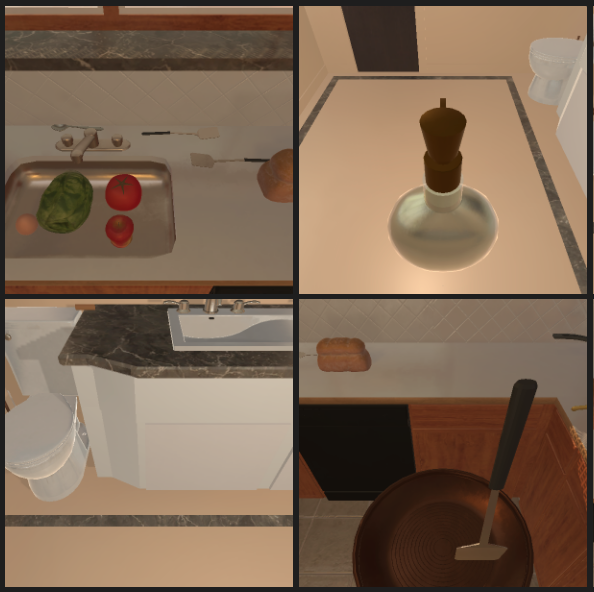
\includegraphics[width=\textwidth]{figures/rgb.png}
         \caption{}
     \end{subfigure}
     \hfill
     \begin{subfigure}[b]{0.32\textwidth}
         \centering
         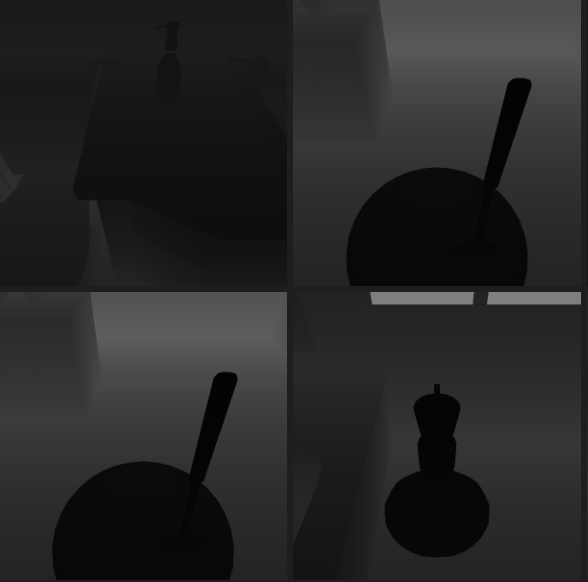
\includegraphics[width=\textwidth]{figures/depth.png}
         \caption{}
     \end{subfigure}
     \hfill
     \begin{subfigure}[b]{0.32\textwidth}
         \centering
         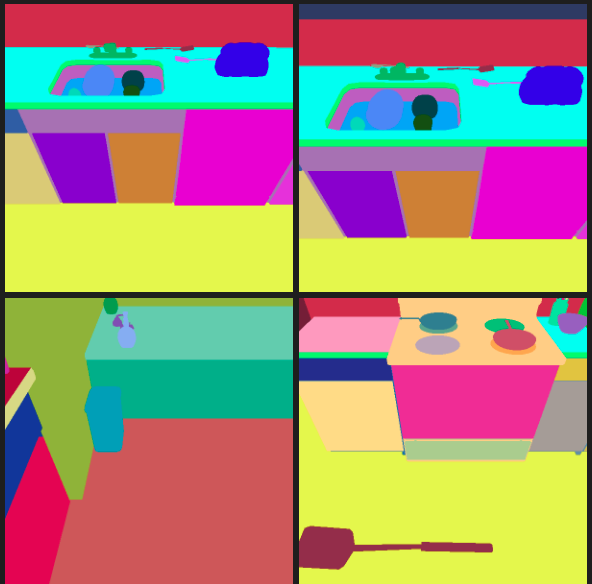
\includegraphics[width=\textwidth]{figures/seg.png}
         \caption{}
     \end{subfigure}
        \caption{Sample RGB, depth, and instance segmentation images retrieved from AI2Thor simulator}
        \label{fig:sample_ims}
\end{figure*}


% can a human do that?
\paragraph{Task solvability} In addition to the quantitative analysis, we also analyzed the solvability of the task. Figures \ref{fig:focus} and \ref{fig:dest} show that the unseen split of the validation set contains objects from the same classes as the training data, but could contain novel instances of those objects in novel environments. Since classes remain the same during training and testing times, the training data contains full information to solve the task, meaning a sufficiently intelligent agent should be able to solve the task, given training data.

\begin{figure*}
    \centering
    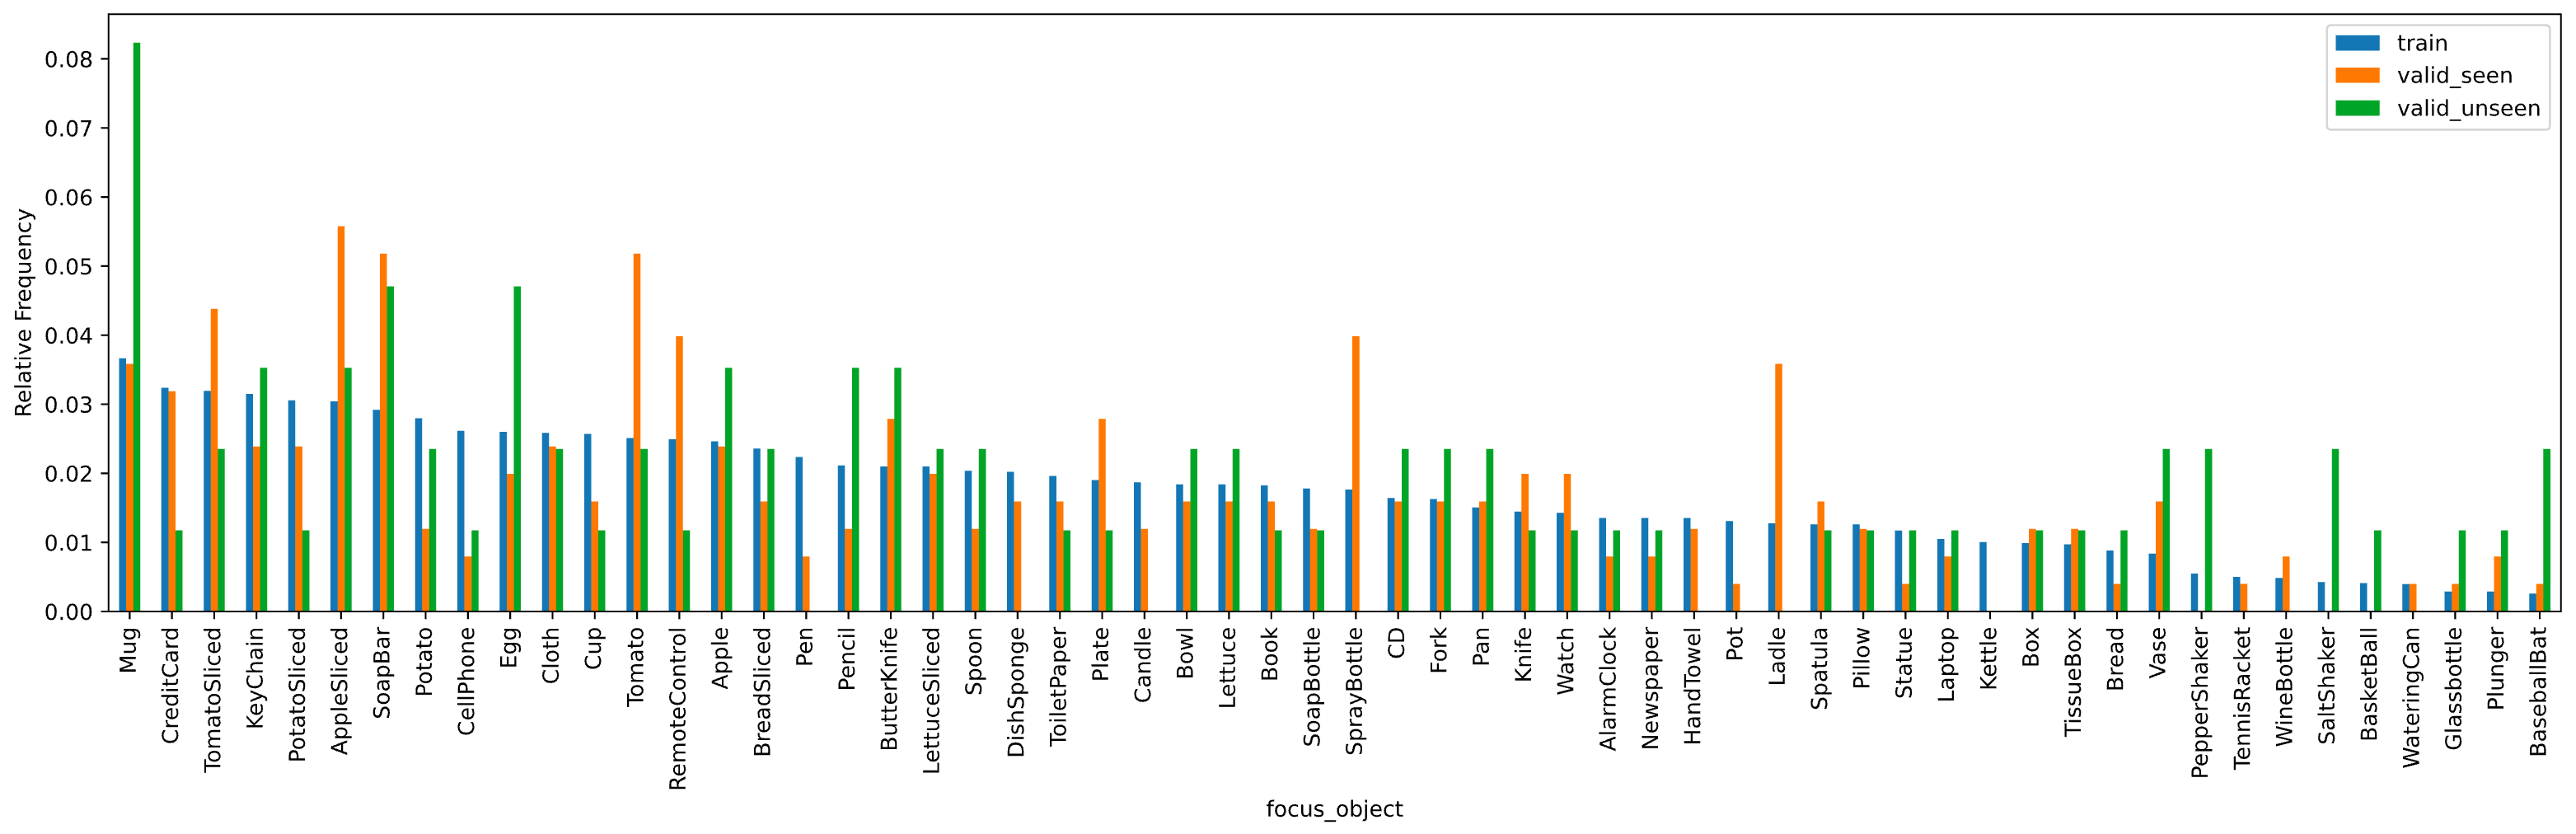
\includegraphics[scale=0.3]{figures/focus_obj_freqs.png}
    \caption{Relative frequency of focus objects used in different splits}
    \label{fig:focus}
\end{figure*}

\begin{figure*}
    \centering
    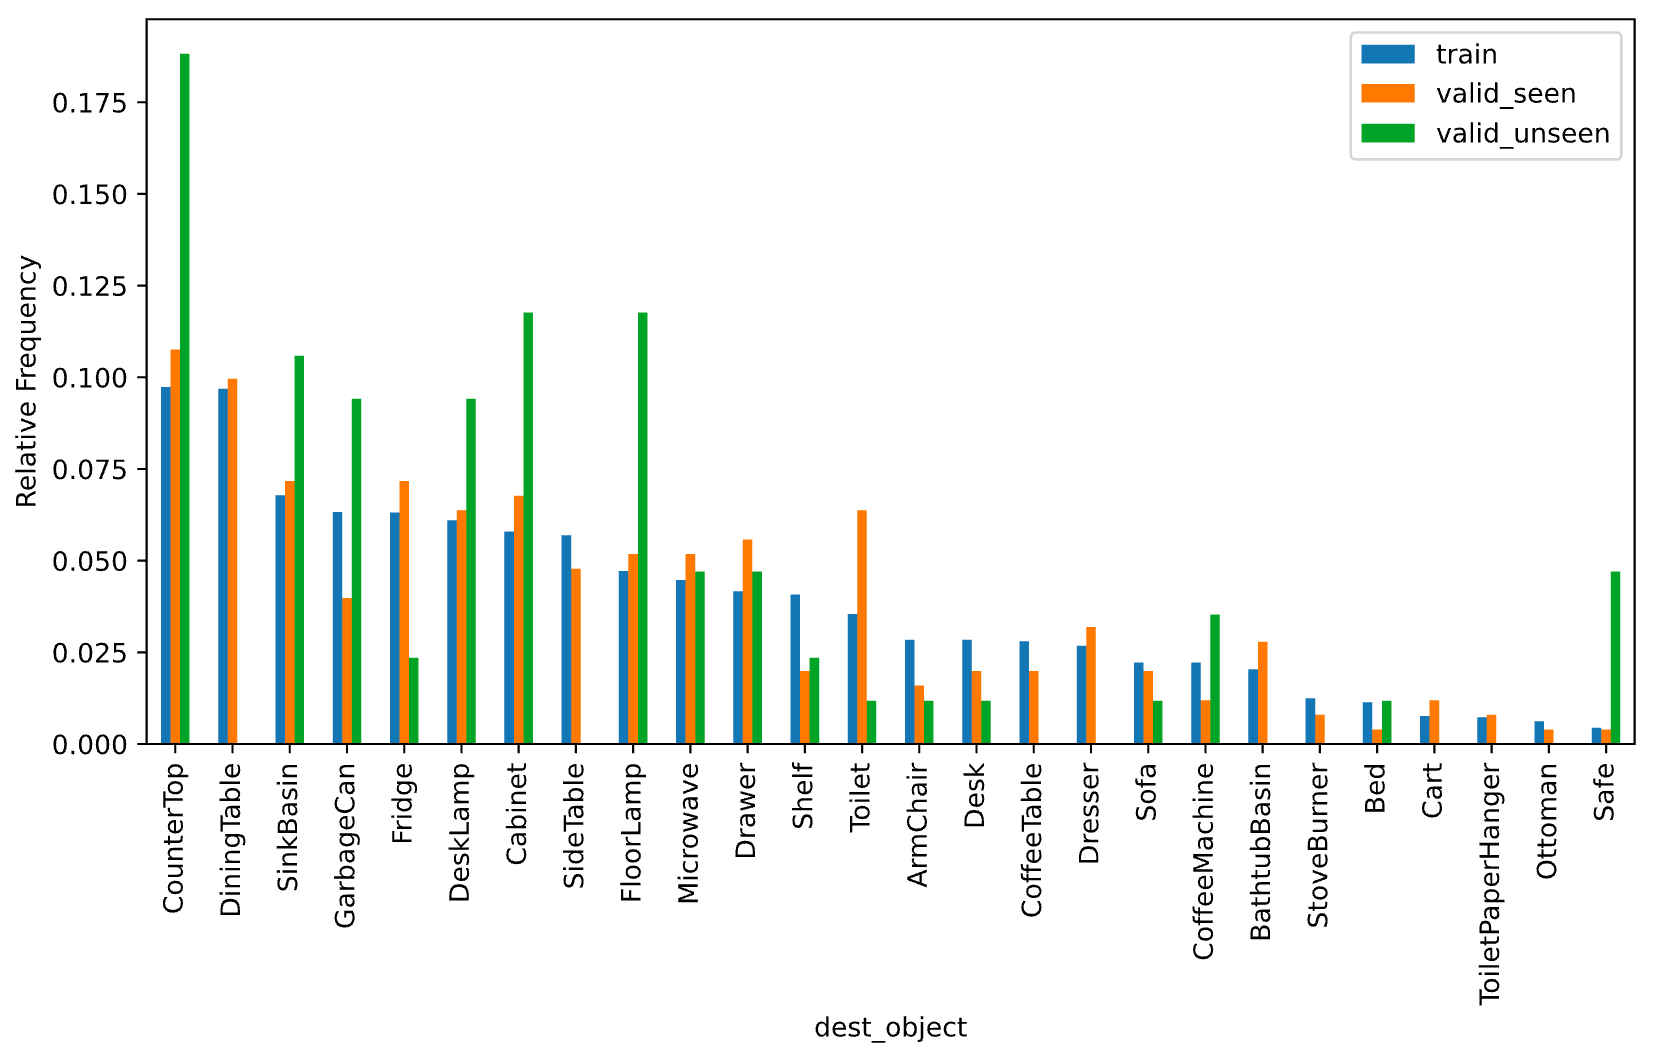
\includegraphics[scale=0.5]{figures/dest_obj_freqs.png}
    \caption{Relative frequency of destination objects used in different splits}
    \label{fig:dest}
\end{figure*}

\subsection{Hard to compute baselines/metrics}
\label{app:missed}
In the following, we list out all baselines/metrics that we planned to run, but could not due to reasons listed below.

\begin{itemize}
    \item \textbf{Seq-2-Seq (CNN-LSTM)} \cite{shridhar2020alfred} We did not evaluate the vanilla CNN-LSTM Seq2Seq architecture because a) we evaluated the progress monitoring variant that gets better performance, and b) the pre-trained model for this was not provided and we wanted to spend our limited compute on better performing models like MOCA \cite{singh2020moca}.
    \item \textbf{Modular Seq-2-Seq} \cite{corona2020modularity} We did not evaluate our internal metrics on the modular Seq2Seq architecture because their code was not released.
    \item \textbf{Seq-2-Seq RL (proposed):} Seq2Seq RL was an architecture we had originally proposed which basically used reinforcement learning to train the policy network which was same as the Seq2Seq PM architecture. However, we were not able to evaluate on this because of several reasons. One, we did some calculations on GPU compute and realized that training using RL would be very expensive which we would not be able to afford (at least not on models that we have not built). Two, we felt that the reward function would need to be heavily tuned to get any satisfactory performance, which would take a lot of time and probably not be considered a "baseline" model since we would have heavily modified it. Three, many libraries/implementations did not support recurrent policies which was just another challenge in implementing this.
    \item \textbf{Interaction Mask Prediction Performance (IMPP)}: We initially defined IMPP as the intersection over union score of the predicted instance segmentation mask with respect to the ground truth mask when the interaction action was correct. The idea was that conditioning on correctness of interaction action would make IMPP only measure the performance of the component that predicts the interaction mask. However, we could not compute this because there was no objective, non-heurestic based way to identify which object the agent intended to interact with at which time. Just matching expert action and predicted at each time step would be too naive because it is unlikely that the agent would mimic the expert so closely.
    \item \textbf{Length-conditioned Success (LCS)}: We initially wanted to compute LCS, which was supposed to be the first $n$ sub-goals successfully completed continuously. However, we could not compute this because the simulator does not store the ordering of the sub-goals, so we could not tell which sub-goals were first and which were last.
\end{itemize}

\subsection {Additional analysis of previous models}
This section includes further analysis of the methods we compare our approach to. The main analysis can be found in Section \ref{sec:prev-models}.
\paragraph{Task-Level Metrics by Task Type}
We group the two task-level metrics, Task Success and Goal-Condition Success, by the 7 task types in ALFRED and plot the results in Figures \ref{fig:ts-by-type} and \ref{fig:gcs-by-type}. While the baseline model struggles with all task types, MOCA demonstrates a substantial improvement on all tasks in the seen split except on the \textbf{Stack \& Place} task. This could be due to the fact that \textbf{Stack \& Place} is the only task with a movable receptacle, presenting a unique challenge that is not found in other tasks. 

The task that both models perform best on is the \textbf{Clean \& Place} task. In the unseen split, MOCA interestingly performs much better on this task than on any other task type. Further exploration of the unique attributes of this task may be needed to determine why MOCA's success rate is so much higher on the unseen split than other tasks. Perhaps it is because this task has less change from seen to unseen than the other tasks, or perhaps it is simply due to variability in the evaluation: the raw number of successes for MOCA on this task in the unseen split was just 18, and was 1-5 for the other tasks.

The key insight from these plots is that for many task types, a substantial improvement in seen performance does not necessarily imply the same improvement in unseen performance. Learning how to successfully generalize to new environments and objects is a distinctive challenge and must be addressed explicitly when designing an approach.

\textbf{We also did a similar task level analysis on metrics we designed ourselves (not discussed due to space constraints), and the results of the same are provided in a \href{https://github.com/ankit61/group-tars-alfred/blob/main/Reports/4-Analysis-of-Baselines/results_analysis.ipynb}{Jupyter notebook} added in the submission folder.}

\begin{figure}[H]
\centering
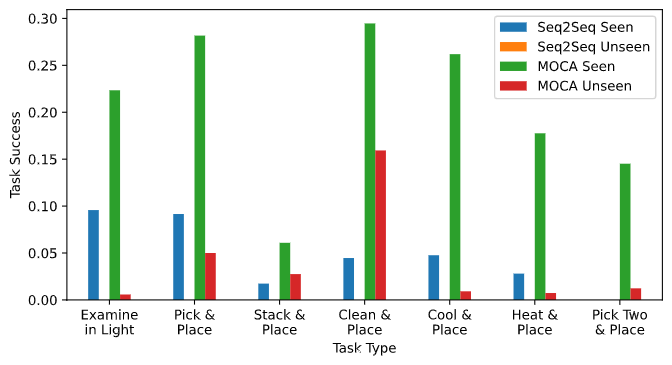
\includegraphics[scale=0.33]{figures/ts_by_type.png}
\caption{Task Success by Task Type}
\label{fig:ts-by-type}
\end{figure}

\begin{figure}[H]
\centering
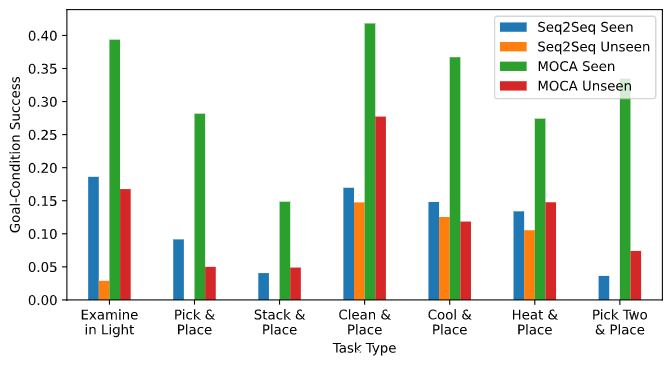
\includegraphics[scale=0.33]{figures/gcs_by_type.png}
\caption{Goal-Condition Success by Task Type}
\label{fig:gcs-by-type}
\end{figure}

\paragraph{Benefit of RL} While we did not get a chance to pursue reinforcement learning for our approach under the current time constraints, an important lesson we learned from our analysis in Section \ref{sec:prev-models} was just how beneficial RL could be for this task. Below we highlight specific reasons we think that RL is useful for solving a multimodal navigation and interaction task like ALFRED:

\begin{enumerate}
    \item Our qualitative analysis highlights cases where the agent makes one mistake and cannot recover from it because it has deviated too much from the expert trajectory and does not have enough information to get back on the right course. This is a common problem that imitation learning agents face \cite{ross2011reduction}, and something RL agents typically won't suffer from because they are trying to maximize a reward instead of rote learn a trajectory.
    \item Since supervision in RL comes from a self designed reward function, we can force the agent to learn much more task specific knowledge compared to the vanilla imitation learning. For example, Table \ref{tab:intrinsic} shows that in most cases agents trained with both MOCA and baseline agents interact with more unnecessary objects than the total objects needed to complete the task (because Unnec-Int is often greater than 1). This is of course an undesirable behavior, but one that cannot be controlled by imitation learning directly. In case of RL, we could simply give a negative reward to the agent for all unnecessary interactions, making the agent explicitly learn that such behavior is undesired.
\end{enumerate}


\subsection{Pipeline features}
\label{app:code}

\begin{enumerate}
    \item Our pipeline uses very strong software engineering and object oriented design principles and strongly decouples all different parts that are logically distinct. Such decoupling allows models in our pipeline to be run without relying on any preprocessing or external dependencies.
    \item Currently, our pipeline supports both the baseline Seq2Seq model and MOCA under a unified interface, which will not only help us compare our model with them, but also all future researchers working on ALFRED who want to compare their models to other SOTA models.
    \item We also have built a Gym style \cite{brockman2016openai} environment for ALFRED, making it amenable to be trained using reinforcement learning easily.
    \item A strong component in helping us keep our code very clean is our custom designed solution for configuration management, which keeps all configuration variables and utility functions separate from the main code, essentially helping us achieve disentanglement between logically separate parts.
\end{enumerate}


\begin{figure*}
    \centering
    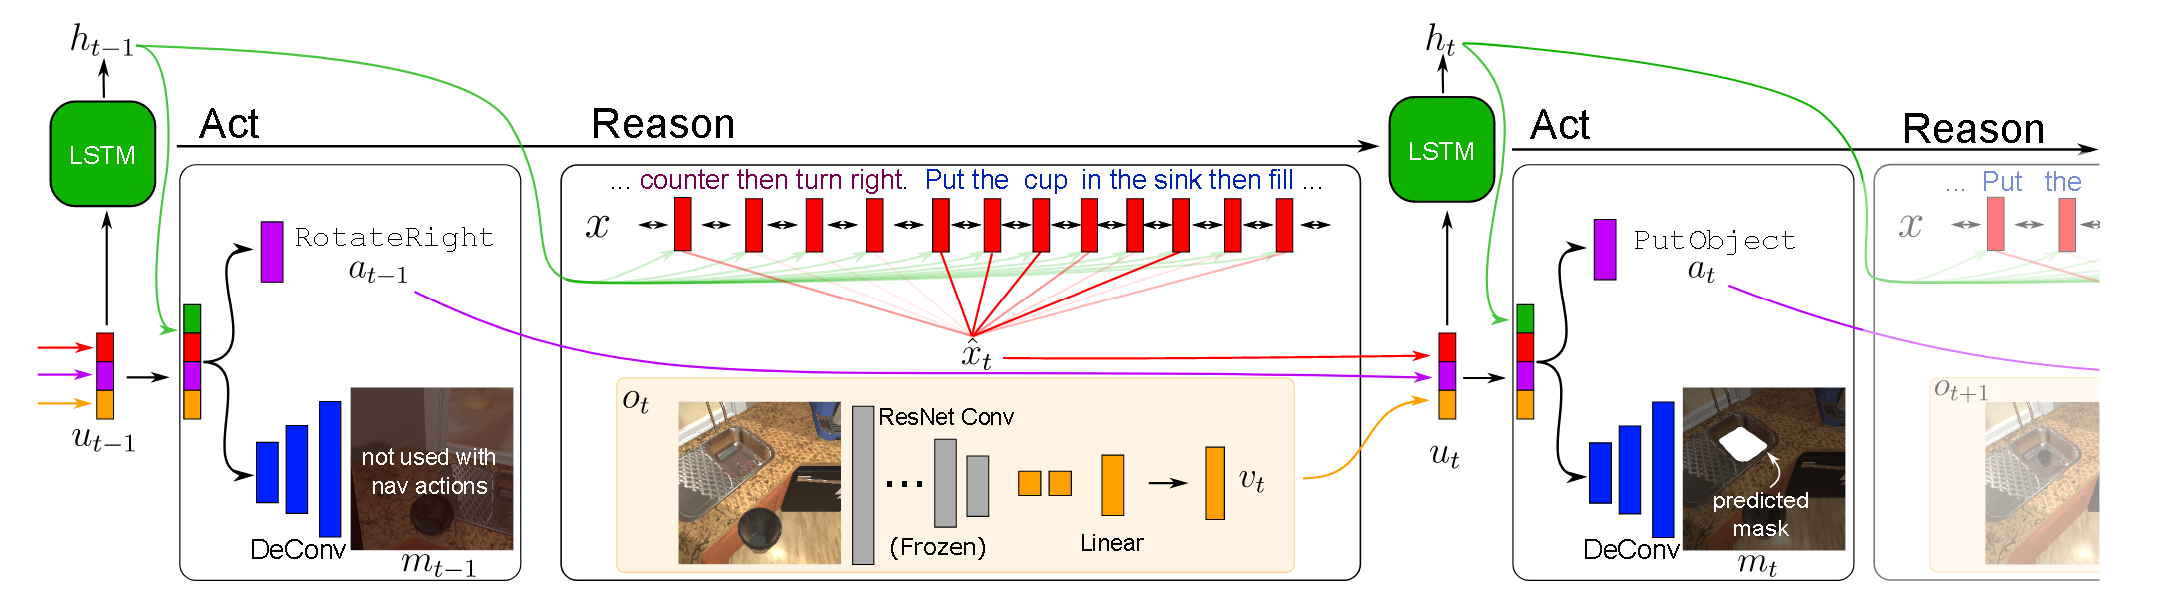
\includegraphics[scale=0.75]{figures/alfred_model.png}
    \caption{ALFRED Baseline Model \cite{shridhar2020alfred}}
    \label{fig:alfred_model}
\end{figure*}

\begin{figure*}
    \centering
    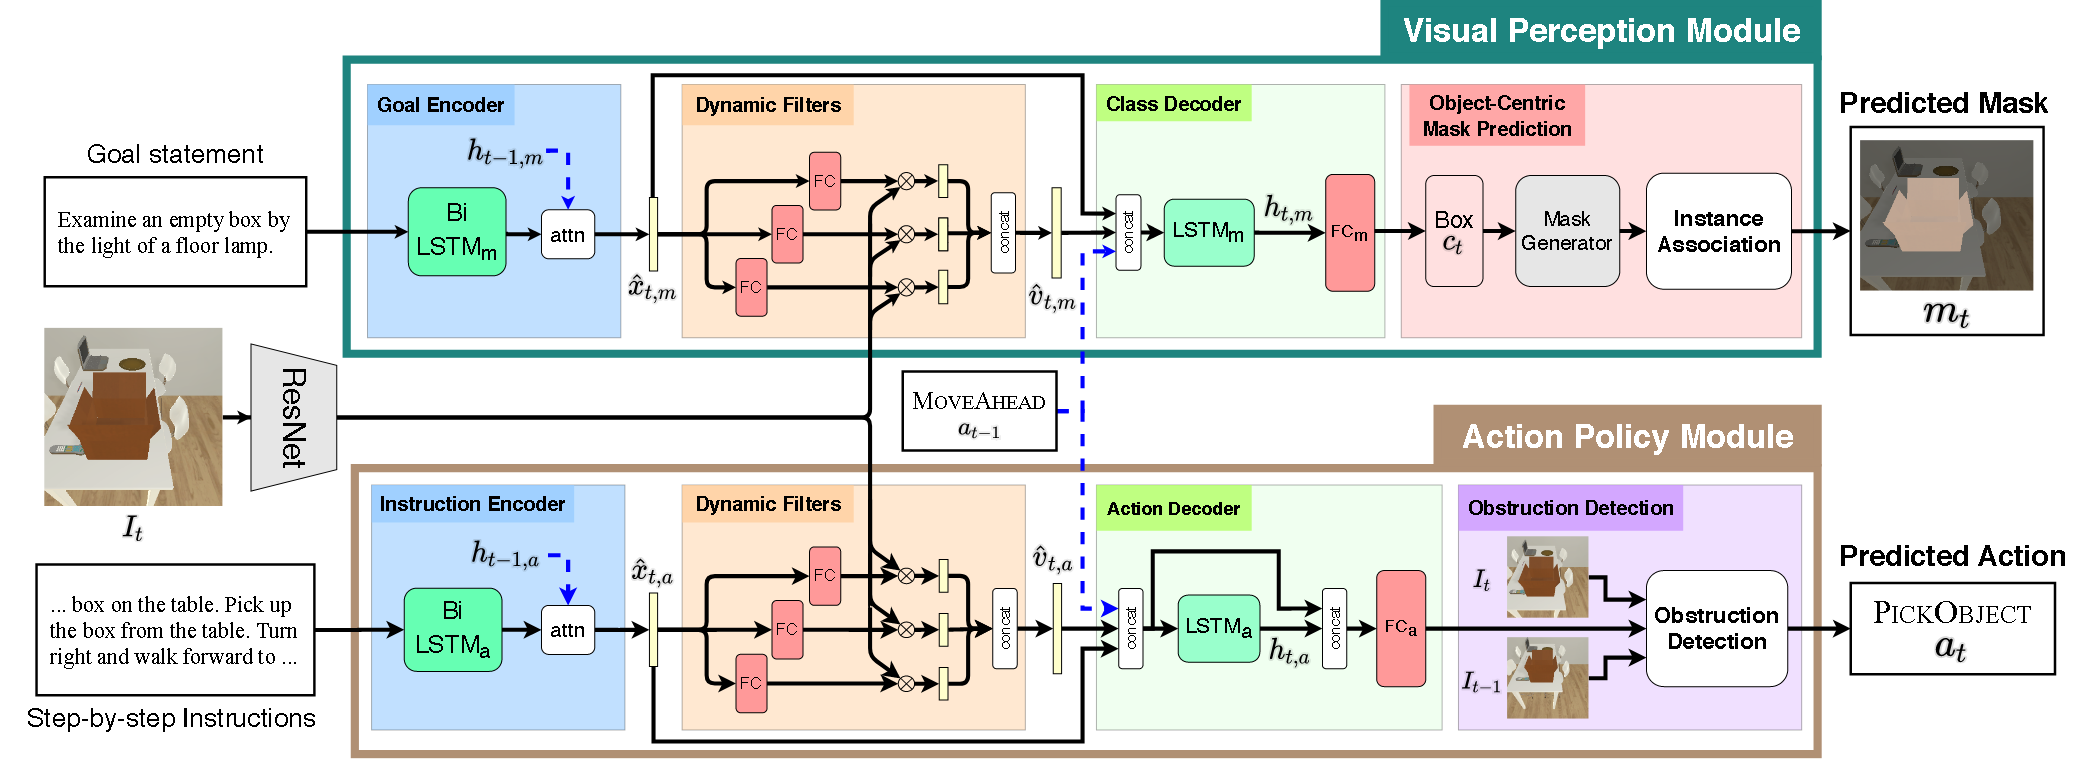
\includegraphics[scale=0.75]{figures/moca_model.png}
    \caption{MOCA Model \cite{singh2020moca}}
    \label{fig:moca_model}
\end{figure*}

% \subsection{Other noteworthy details}
% We want to highlight that there were certain baseline models and metrics that we had planned to do in this submission, but could not due to various reasons such as implementation feasibility, compute limits, etc. We explain specific reasons why those baselines and metrics could not be computed in the appendix Section \ref{app:missed}.

% Moreover, we want to highlight that we built a full end to end pipeline to perform our analysis, which contains clean, refactored and generalizable  versions of the baseline Seq2Seq model \cite{shridhar2020alfred} and MOCA \cite{singh2020moca}. The current implementation of the baseline Seq2Seq model \cite{shridhar2020alfred} is quite complicated and very tightly intertwined with specific other code in their library. These factors implicitly force all other ALFRED models to be coded up in a very specific manner, so they can use the evaluation scripts provided by the original ALFRED authors. For example, the MOCA model is also implemented using same ALFRED code because of tight coupling within different parts in that code base (such as dependence of models on specific styles of data preprocessing).  We feel this is suboptimal because such coding styles hinder generality. For example, it is not (easily) possible in the original code base to train the same proposed baseline model as a policy network using reinforcement learning. Therefore, we designed our pipeline that can take any model and potentially train it using both reinforcement learning and/or imitation learning. We want to highlight that the actual training code has not be written because that was not the goal of this milestone, but the interface is generic enough to support it. We highlight important features of our pipeline in appendix Section \ref{app:code}.


\subsection{Additional methods and experimental findings}
\label{ssec:add-exp}
\paragraph{Hidden Bugs} 
Initially, we were struggling a lot to make the model converge even on a single demonstration, and it was unclear if our idea was fundamentally flawed, or whether there were bugs in our implementation. After thorough testing, we found out three hidden bugs in our models. Specifically, we were missing a few non-linearities after some attention layers which was significantly hurting our model expressivity, our hidden state management had some flaws which was not letting our action module receive proper hidden states leading to context not being updated correctly, and our contextual embeddings were stochastic because of an incorrect token being passed. While such bugs naturally arise in any large and complex models, we just highlight them here because finding them took very significant time.

\paragraph{Readout transformer pretraining}
We hypothesized that the transformers in our Context Module (Figure \ref{fig:model}) may not receive sufficient learning signal during end-to-end training of our model due to the longer path that gradients need to take relative to our core Action Module. We attempted to alleviate this issue by pretraining these transformers with a reconstruction objective so that prior to end-to-end training, these transformers would already be capable of producing somewhat meaningful representations of the agent's action and interact object histories respectively. We can view each transformer as a sequence encoder, computing an embedding for a sequence of previous actions or previous interaction objects. During pretraining, we add an LSTM decoder whose hidden state is initialized to the transformer's output, and we task the decoder to auto-regressively predict the original sequence encoded by the transformer. We supervise the decoder's predictions with a standard cross-entropy loss, where the classes are either the actions or the interaction objects. Using the expert trajectories as training data, we jointly train the transformer encoder and LSTM decoder on this reconstruction objective. Our initial results from this pretraining were promising: the action history transformer achieved over 99\% accuracy on both splits of the validation dataset, and the interaction object history transformer over 87\% accuracy, where we measure accuracy as $\frac{\sum_{i=1}^N \mathbbm{1}_i}{N}$ where $N$ is the sequence length and $\mathbbm{1}_i$ is the indicator variable denoting whether the $i^{th}$ prediction is correct (we explicitly task the decoder with making $N$ predictions rather than having it decide when the predicted sequence should end). While the sequence lengths for both action and interaction object histories were the same, we hypothesize that the higher performance for action history is due to the fact that there are many more object classes than action classes (119 vs. 13). 

Unfortunately, due to the fact that the late stages of our model tuning involved changes to the embedding size and depth of these transformers, we were not able to make use of this pretraining procedure in our final model. We leave further exploration of this component as future work.


\end{document}
